\documentclass[11pt]{article}
\usepackage[T1]{fontenc}
\usepackage{lmodern}
\usepackage[margin=1in]{geometry}
\usepackage{amsmath,amssymb}
\usepackage{graphicx}
\usepackage{booktabs}
\usepackage{array}
\usepackage{float}
\usepackage{xcolor}
\usepackage[hidelinks]{hyperref}

\newcommand{\Xp}{X_{0.99}}
\newcommand{\xs}{x^{*}}
\setlength{\parskip}{0.45em}
\setlength{\parindent}{0pt}

\title{\vspace{-3.2em}Detecting and quantifying change in extremes:\\a synthetic-data test of the M\"uller--Watson methods}
\author{Produced by Ken Caldeira with the help of Claude Code \\ \small\url{https://github.com/Sustainable-Solutions-Lab/extreme-trend-detection}}
\date{Draft, 4 November 2026}

\begin{document}
\maketitle
\vspace{-2.5em}

\section*{Abstract}

\emph{Questions and approach.} We asked four questions about the methods of M\"uller and Watson
(2024) for extremes that change over time:
\vspace{-0.6\baselineskip}
\begin{enumerate}\setlength{\itemsep}{0pt}\setlength{\parskip}{0pt}
\item How reliably do they detect a change?
\item How accurately do they estimate the current 1-in-100-year level?
\item What happens when the model of the change is wrong?
\item How close to the true risk is their Bayesian model's posterior-predictive 1-in-100-year
  level, which builds in parameter uncertainty, and why?
\end{enumerate}
\vspace{-0.4\baselineskip}
\noindent To answer them against a known truth, we generated synthetic daily records of 30 to 150 years from
four distributions (temperature-like, precipitation-like, heavy-tailed and bounded), changed their
mean, spread or tail in known ways, and applied the tests and estimators to the annual maxima:
thousands of records per case for the tests and 100 per case for the estimates
(Table~\ref{tab:design} lists the dimensions varied).

\emph{Detection.} The parameter-constancy (Nyblom) test of M\"uller and Watson (2024) is a reliable
detector of change in annual maxima: with one value per year its false-alarm rate stays at
4--6\% for every parent distribution, record length and level of day-to-day persistence we tried.
Its power depends strongly on the record length and on the shape of the daily distribution. A
mean shift of half a daily standard deviation over the record is detected in 89\% of 85-year
records from a normal parent but in 24\% from a skewed, precipitation-like (gamma) parent, and in
41\% and 9\% of 30-year records. With one value per year, however, it is no more powerful than the
simpler Mann--Kendall rank test, which detects change about as often or more often in almost every
case we simulated; the Nyblom test pulls ahead when it uses the three largest values per year, which
must then be declustered.

\emph{Quantification.} Saying how large the change is, or what the current 1-in-100-year level
is, is much harder. Even with no change and the correct model, the 99\% annual-maximum level
estimated from 85 years is badly off in 44\% of records, in the sense that its true chance of being
exceeded is more than twice or less than half the nominal 1\%: it understates the risk in 27\% of
records and overstates it in 18\%. When extremes are changing, the methods we tested, including the
authors' Bayesian random-walk model, are badly off in 51--59\% of 85-year records and in about
three-quarters of 30-year records. The Bayesian model's posterior median is no more accurate than a
simple linear trend.

\emph{Using the wrong model.} Change can be modelled as a function of time or of the mean state;
which is right is usually unknown, the record rarely shows it, and the wrong choice matters most
when the mean changes nonlinearly or the spread changes without the mean. Averaging the candidate
models, weighted by how well each fits, comes close to the best single model whatever the truth.

\emph{The posterior-predictive level.} Taking the 99th percentile of the Bayesian model's posterior
predictive distribution, rather than the median of the draws' levels, gives a level that is right or
conservative on average (true exceedance 0.8\% at 85 years, 0.4--0.6\% at 30--45 years) and rarely
understates the risk. In a single record, however, it usually overstates the risk, often by a lot:
its typical true exceedance is 0.4\%, 0.05\% and 0.01\% at 85, 45 and 30 years, and it misses
twofold in 68\%, 84\% and 92\% of records. Its uncertainty comes from the short record and the
prior, not from the computation, and it is as large in records with no change at all.

\setcounter{tocdepth}{1}
\tableofcontents
\newpage

%=====================================================================================
\section{Questions}

M\"uller and Watson (2024) develop small-sample inference for extremes whose parameters may change
over time: likelihood-ratio tests about the GEV parameters (the tail index, a high quantile, a
Pareto tail) and the Nyblom test of parameter constancy, both with critical values that depend on
the estimated tail index, and a Bayesian time-varying GEV model with random walks in its
parameters, estimated by Hamiltonian Monte Carlo. They apply the methods to weather-disaster
damages, stock returns, and city and firm sizes. Their simulations calibrate the size of the tests
for data drawn exactly from the GEV model. They do not report power, do not test the methods on
data whose extremes are only approximately GEV (the usual situation), treat serial dependence only
briefly (an appeal to weak-dependence results and one simulation for the city-size data), and do
not check whether the Bayesian model recovers known parameter paths. For climate applications these are the questions that
matter:

\begin{enumerate}
\item \textbf{Detection.} How often is a change of realistic size detected with record lengths
  typical of reanalyses and stations (30, 45, 85 and 150 years), and how often is a change
  ``detected'' when there is none?
\item \textbf{Quantification.} How well do the methods estimate the current return level, for
  example the level the annual maximum exceeds with probability 1\% this year ($\Xp$), and its
  change over the record? Each method gives a best estimate of this fixed but unknown level; for
  the Bayesian model it is the posterior median.
\item \textbf{Using the wrong model.} A change can be modelled as a function of time (trends,
  random walks) or of the mean state (a covariate). Either could be physically right, and usually
  we do not know which. What is lost when the change follows one and we model it as a function of
  the other, and what can be done when we do not know?
\item \textbf{The posterior-predictive level.} A Bayesian user who must price risk reports the
  99th percentile of the posterior predictive distribution rather than a statistic of the
  posterior draws. That level is not an estimate of $\Xp$: it is the level whose chance of being
  exceeded is 1\% once parameter uncertainty is averaged in. How close is it to the true risk,
  and where does its uncertainty come from?
\end{enumerate}

%=====================================================================================
\section{Methods}

\subsection{Study design at a glance}

Table~\ref{tab:design} lists the dimensions we varied. It is not a full factorial: the persistence
and values-per-year variations were run mainly at 85 years, and the quantification study uses one
size of change per case.

\begin{table}[H]
\centering
\small
\renewcommand{\arraystretch}{1.15}
\begin{tabular}{>{\raggedright\arraybackslash}p{0.19\textwidth}>{\raggedright\arraybackslash}p{0.36\textwidth}>{\raggedright\arraybackslash}p{0.36\textwidth}}
\toprule
 & \textbf{Detection} (is there a change?) & \textbf{Quantification} (what is the current 99\% level?) \\
\midrule
Daily distribution (parent) & \multicolumn{2}{>{\raggedright\arraybackslash}p{0.74\textwidth}}{normal (temperature-like); gamma, shape 2 (precipitation-like); Student-$t$, 6 d.f.\ (heavy-tailed); beta(4,\,4) (bounded)} \\
What changes & mean; width; tail (gamma, $t$, beta); position within the bounds (beta) & the same, plus covariate-model cases (width and tail follow the mean; precipitation scaling) and their time-driven counterparts \\
Shape of the change & none; linear; step at mid-record; step at 80\% of the record; accelerating & none; linear; step at mid-record; accelerating \\
Size of the change & four sizes per feature (e.g.\ mean shift 0.1--1.0 daily sd) & one size per feature (e.g.\ mean shift 0.5 daily sd) \\
Record length & 30, 45, 85, 150 years & 30, 45, 85 years \\
Values per year & 1, 3 (all lengths); 10 (85 years) & 1; 3 (45 and 85 years) \\
Declustering & none; values at least 3 days apart (10 per year) & values at least 3 days apart (3 per year) \\
Day-to-day persistence (AR(1) $\phi$) & 0.5; 0 and 0.8 at 85 years & 0.5; 0 at 85 years \\
Methods & Nyblom test (M\"uller--Watson), location-trend LR test, two-halves test, Mann--Kendall & 14 estimators: constant, last 30 years, two halves, location trend, location + width trend, all-parameter trend, mean-state covariate (two forms, and oracles with the true mean), AIC choice, AIC-weighted average, Bayesian random walks (posterior median and mean) \\
Bayesian prior & --- & authors'; tighter (45 and 85 years) \\
Records per case & 10,000 with no change; 2,000 per change & 100 \\
Scores & false-alarm rate (size); detection rate (power) & true exceedance probability of the last year's estimated level: missed $>2\times$ either way, understated, overstated; error in the estimated change; Bayesian interval coverage and width \\
\bottomrule
\end{tabular}
\caption{Study design. Columns: the detection study (does a test find a change?) and the quantification study (how close is the estimated current 1-in-100-year level to the truth?). Rows: the dimensions varied. Not every combination was run: persistence and values-per-year variations were run mainly at 85 years.}
\label{tab:design}
\end{table}

\subsection{Extremes model and tests}

For each year $t=1,\dots,T$ we keep the $k$ largest daily values
$X_t^{(1)}\ge\dots\ge X_t^{(k)}$ (with $k=1$, the annual maximum). By extreme-value theory these
follow approximately the GEV$_k$ distribution with location $\mu$, scale $\sigma$ and shape
(tail index) $\xi$, with density
\[
f(x_1,\dots,x_k)=\sigma^{-k}\exp\!\Big[-(1+\xi z_k)^{-1/\xi}\Big]\prod_{j=1}^{k}(1+\xi z_j)^{-1/\xi-1},
\qquad z_j=\frac{x_j-\mu}{\sigma}.
\]
The tests compared are:
\begin{itemize}
\item \textbf{Nyblom} (M\"uller and Watson, eq.~12; Nyblom, 1989): with scores $S_t$ of the
  constant-parameter fit and average information $V$,
  $L_T=T^{-2}\sum_t\big(\sum_{l\ge t}S_l\big)'V^{-1}\big(\sum_{l\ge t}S_l\big)$. The test rejects
  when $L_T\exp(a_0+a_1\hat\xi+a_2\hat\xi^2)>1$, with coefficients calibrated by simulation so that
  the rejection rate is at most 5\% for every true $\xi$ on a grid and otherwise as close to 5\% as
  possible (their Appendix~B: ten values of $\xi$ in $[-0.5,1.5]$). We recalibrated the
  coefficients in the same way for each record length and $k$ used here, with 40,000 simulated
  null records per grid value (they used 10,000).
\item \textbf{Location-trend LR}: GEV with $\mu_t=\mu_0+\mu_1 t$, likelihood-ratio test of
  $\mu_1=0$ against $\chi^2_1$. This is the standard tool in climate science (e.g.\ Coles, 2001).
\item \textbf{Two halves}: separate GEV fits to the first and second halves of the record, LR
  test of equal parameters, critical values calibrated like the Nyblom test.
\item \textbf{Mann--Kendall} rank test for a monotone trend in the annual maxima.
\end{itemize}

\subsection{Estimators of the 99\% level}

Each estimator gives a path $\hat X_{0.99}(t)$, the level the annual maximum of year $t$ exceeds
with probability 1\% (the 100-year return level in that year's climate). All are fitted by
maximum likelihood to the same records, except the Bayesian model.
\begin{description}
\item[Constant] GEV with constant parameters (ignores change).
\item[Last 30 years] constant GEV fitted to the most recent 30 years only, a common practical
  shortcut (equal to the constant fit for 30-year records).
\item[Two halves] constant GEV fitted to the second half of the record.
\item[Location trend] $\mu_t$ linear in time, $\sigma$ and $\xi$ constant.
\item[Location + width trend] $\mu_t$ and $\log\sigma_t$ linear in time, $\xi$ constant.
\item[All-parameter trend] $\mu_t$, $\log\sigma_t$ and $\xi_t$ linear in time.
\item[Mean-state covariate] $\mu_t$ and $\log\sigma_t$ linear in $c_t$, $\xi$ constant, where
  $c_t$ is a smoothed annual mean of \emph{all} daily values (local-linear smoother, Gaussian
  kernel, bandwidth 10 years, fixed in advance). This is the usual approach in event attribution,
  where the covariate is a smoothed (global or local) mean temperature (Philip et al., 2020). A
  variant with all three parameters linear in the raw annual mean is unstable (the tail index
  follows the year-to-year noise of the covariate) and is shown only for reference.
\item[Covariate (true mean)] as above but with the true mean path as covariate: an oracle that
  shows the cost of estimating the covariate.
\item[Data-chosen (AIC)] for when the form of the change is unknown: of the constant, location-trend,
  location + width trend and mean-state covariate models, the one with the lowest AIC.
\item[AIC-weighted average] the average of the same four models' $X_{0.99}$ paths, with Akaike
  weights $w_i\propto\exp(-\Delta\mathrm{AIC}_i/2)$.
\item[Bayesian] the authors' four-random-walk model (their \texttt{GEV\_4RW\_Model.stan},
  unchanged likelihood and priors), posterior median of $X_{0.99}(t)$. The parameters follow
  random walks in a logistic transform of $\xi_t\in(-0.9,2.1)$, in $\ln\alpha_t$, $\ln s_t$ and
  $m_t$, with $\sigma_t=s_t\alpha_t^{\xi_t}$ and $\mu_t=m_t+(s_t/\xi_t)(\alpha_t^{\xi_t}-1)$.
  The innovation standard deviations are $\gamma=\mathrm{sg}\cdot g/\sqrt T$ with
  $g\sim\mathrm{Exp}(1)$ and scale factors $\mathrm{sg}=1,0.5,0.5$ for $\xi,\alpha,s$ (and the
  scale level for $m$), the prior means the paper calls $g$ (their eq.~15). We use 4 chains of
  1,000 warm-up and 1,000 sampling iterations (\texttt{adapt\_delta} 0.95, against Stan's default of
  0.8 in the authors' runs); the authors used 5,000 and 10,000 for single published fits. Like
  their replication scripts, we use the draws without the importance-sampling correction for the
  extended-support likelihood described in their Section~3.2.3, whose weights they report to be
  essentially 1. We
  also report the posterior mean, the 99th percentile of the posterior predictive distribution
  (Section~\ref{sec:pred}), and a run with a tighter prior ($\mathrm{sg}=0.25$ for all three).
\end{description}

\subsection{Synthetic data}

A daily standard Gaussian series $Z_d$ with AR(1) correlation $\phi$ (0.5 unless stated; 0 and
0.8 also run) is mapped through the parent's quantile function,
$X_d=m_t+s_t\,\varepsilon(Z_d;\text{tail}_t)$, with $m_t$, $s_t$ and the tail parameter constant
within a year. The parents are standardized so that the baseline daily standard deviation is 1;
all levels are in these units. For a daily temperature with a standard deviation of 3--4\,K, a
change of 0.5 is 1.5--2\,K.

\begin{center}
\small
\begin{tabular}{llll}
\toprule
Parent & $\varepsilon$ & Tail parameter (baseline) & Tail of the extremes \\
\midrule
Normal & $Z$ & --- & light, $\xi\to0$ slowly \\
Gamma & standardized gamma($a$) & shape $a=2$ & exponential-type, skewed \\
Student-$t$ & standardized $t_\nu$ & $\nu=6$ & heavy, $\xi=1/\nu$ \\
Beta & $3(2B-1)$, $B\sim\mathrm{beta}(\alpha,\beta)$ & $\alpha=\beta=4$ & bounded, $\xi=-1/\beta$ \\
\bottomrule
\end{tabular}
\end{center}

Because the map from $Z$ to $X$ is increasing within a year, the annual maximum of $X$ is the map
applied to the annual maximum of $Z$, so the true $X_{0.99}(t)$ is known exactly: in closed form
for independent days, and from 500,000 simulated years of $Z$ for correlated days (error about
0.005 at $p=0.99$).

The changes (Appendix, Table~\ref{tab:cases}) move one feature at a time over the record, along
a linear, mid-record step or accelerating path (exponential in time, so the feature changes at an
increasing rate): the mean, the width ($\log s$), the
tail parameter (log of $a$, $\nu$ or $\beta$), or, for the beta, the position of the mass within
fixed bounds. A second set, the \emph{covariate-model cases}, is built so that a mean-state model
is correct:
\begin{itemize}
\item \emph{Temperature-like} (normal, $t$, beta): the mean rises by 0.5 (beta 0.25) along an
  accelerating path, the width follows it ($\log s_t=0.25\,m_t$), and for the $t$ and beta so
  does the tail ($\log\nu_t$ or $\log\beta_t=-0.2\,m_t$, a heavier-tailed $t$ and a more tightly
  bounded beta as it warms).
\item \emph{Precipitation-like} (gamma): the mean is scaled by $\lambda_t=e^{g_t}$ with a 22\% rise
  over the record, so every quantile scales with the mean (a Clausius--Clapeyron-type change);
  in a variant the gamma shape also falls as it gets wetter (heavier tail).
\end{itemize}
A third set, the \emph{time-driven} counterparts of the accelerating temperature-like cases, has the
same mean path and the same first- and last-year distributions, but the width and tail change
linearly in time between those states instead of following the mean (Section~\ref{sec:wrong}).

\subsection{Scoring}

For detection we report the rejection rate at the nominal 5\% level with no change (size) and with
change (power). For quantification, the main score is the \emph{true exceedance probability} of
each record's estimated level in the last year,
\[
\pi=\Pr\big(M_T>\hat X_{0.99}(T)\big),
\]
computed from the exact distribution of the last year's annual maximum $M_T$. An ideal estimator
has $\pi=1\%$. We report its median over records and count an estimate as a \emph{miss} when
$\pi>2\%$ (risk understated at least twofold) or $\pi<0.5\%$ (overstated at least twofold). The main
score is the share of records missed in either direction, always given with its two parts. The two
errors have different consequences: understating the risk leaves people unprepared, overstating it
leads to over-design and false alarms. Estimators trade one for the other, so neither alone is a fair
summary, and when the true change has a known direction a one-sided score rewards models that err in
that direction. This score is comparable across parents and penalizes errors by their consequence
for risk rather than by their size in data units. We also report the error of the estimated change $\hat X_{0.99}(T)-\hat
X_{0.99}(1)$ and, for the Bayesian model, the coverage and width of its 90\% credible intervals.

\subsection{Monte Carlo design}

Detection results (``Stage B'' in the repository) use 10,000 simulated records with no change
and 2,000 per change. Quantification results (``Stage C'') use 100 records per case, fitted by all
estimators. The same
daily noise is used across cases, record lengths and estimators (common random numbers), so
comparisons between estimators are paired. A bootstrap over records gives standard errors of 3--4
percentage points on the pooled shares and about 3 points on differences between estimators.

%=====================================================================================
\section{Detecting change}

\subsection{False alarms}\label{sec:size}

With one value per year, all four tests hold their nominal size within Monte Carlo error at every
record length and persistence level (Figure~\ref{fig:size}), except the location-trend LR test
for short records (7--10\% at $T=30$), where the $\chi^2$ approximation is poor. Using several
values per year from a persistent daily series breaks the independence the GEV$_k$ model assumes:
with the three largest values per year, the Nyblom test rejects 7--9\% at $\phi=0.5$ and 21--23\%
at $\phi=0.8$, and with ten values 46--51\%. Requiring the values to be at least three days apart
(declustering) brings the last case down to 9--12\%. Mann--Kendall uses only the annual maxima
and is unaffected.

\begin{figure}[H]
\centering
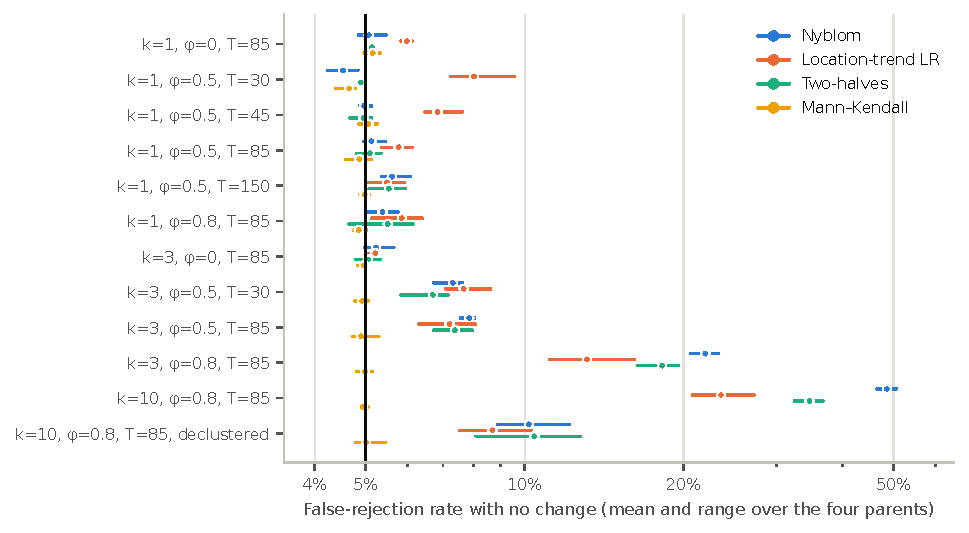
\includegraphics[width=\textwidth]{figures/fig05_size.pdf}
\caption{False alarms: how often each test rejects ``no change'' at the nominal 5\% level when nothing is changing. Rows: designs, given by the number of values used per year $k$ ($k=1$: the annual maximum), the day-to-day correlation $\phi$ of the daily series and the record length $T$ in years; ``declustered'': the values are at least 3 days apart. Dots: mean over the four parent distributions; lines: their range. Vertical line: the nominal 5\%. With one value per year all tests stay near 5\% except the location-trend LR test at 30 years; several values per year from a persistent series raise false alarms (to 20--50\% at $\phi=0.8$) unless they are declustered.}
\label{fig:size}
\end{figure}

\subsection{Power}

Power rises steeply with record length (Figure~\ref{fig:power}, Table~\ref{tab:power}). For a
normal parent, a mean shift of 0.5 daily standard deviations over the record is detected by the
Nyblom test in 41\%, 60\%, 89\% and 99\% of records of 30, 45, 85 and 150 years. The same shift is
much harder to detect for skewed or heavy-tailed parents (gamma: 9--41\%; $t$: 11--52\%), whose
annual maxima are more variable relative to the daily standard deviation. The location-trend LR
test is more powerful against the change it is designed for, a linear shift in location (63\% at
30 years and 96\% at 85 years for the normal mean shift, though part of the edge at 30 years
comes from its over-sizing), but much less powerful against a change in tail shape ($t$ parent:
36\% against 69\% for the Nyblom test at 85 years).

With one value per year the Nyblom test is not the most powerful of the four. The rank-based
Mann--Kendall test, which uses only the annual maxima, does well against both kinds of change (93\%
and 73\% in the two examples). Over all 768 simulated changes with one value per year, with
rejection rates corrected for size, it detects change at least as often as the Nyblom test, to
within a point, in 95\% of cases; the average power is 47\% for Mann--Kendall, 45\% for the
Nyblom and LR tests and 37\% for the two-halves test. The Nyblom test is ahead mainly for steps late
in the record. Its advantage comes with more values per year, which Mann--Kendall cannot use: with
the three largest values per year (size-corrected) it detects change at least as often as
Mann--Kendall in 94\% of cases (average 56\% against 47\%), and more often than the LR test for tail
changes (49\% against 39\%). In a persistent daily series these values must be declustered to hold
the false-alarm rate (Section~\ref{sec:size}).

\begin{figure}[H]
\centering
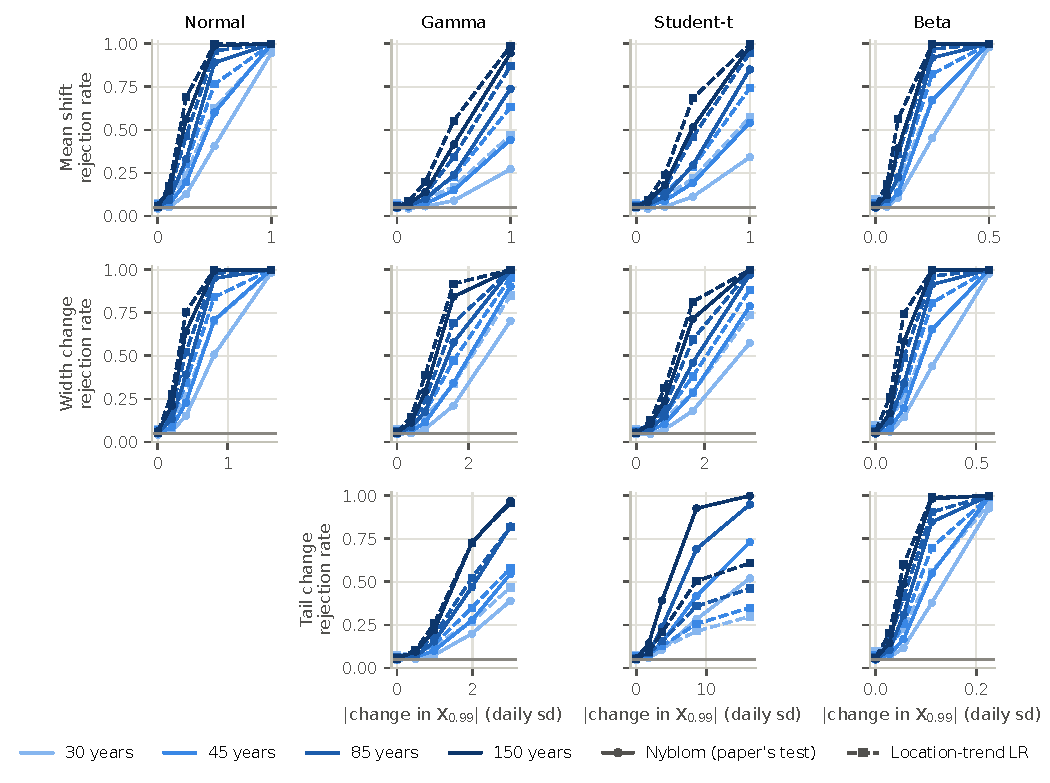
\includegraphics[width=\textwidth]{figures/fig04_power.pdf}
\caption{Detection rate: the share of records in which a test rejects ``no change'' at the nominal 5\% level, against the size of the true change in the 1-in-100-year level $\Xp$ over the record (in baseline daily standard deviations; computed for independent days, within 1\% of the correlated-day value). Rows: linear change in the mean, width or tail of the daily distribution; columns: parent distribution (the normal has no tail parameter). Colour: record length, light (30 years) to dark (150). Solid, circles: Nyblom test (the paper's); dashed, squares: location-trend likelihood-ratio test. Grey line: 5\%. One value per year, day-to-day correlation 0.5. The same change is detected far less often for skewed or heavy-tailed parents than for the normal.}
\label{fig:power}
\end{figure}

\begin{table}[H]
\centering
\scriptsize
\setlength{\tabcolsep}{2.6pt}
\begin{tabular}{llrrrrrrrrr}
\toprule
 & & & \multicolumn{2}{c}{$T=30$} & \multicolumn{2}{c}{$T=45$} & \multicolumn{2}{c}{$T=85$} & \multicolumn{2}{c}{$T=150$} \\
\cmidrule(lr){4-5} \cmidrule(lr){6-7} \cmidrule(lr){8-9} \cmidrule(lr){10-11}
Parent & Change & $\Delta X_{0.99}$ & Nyb. & LR & Nyb. & LR & Nyb. & LR & Nyb. & LR \\
\midrule
Normal & mean 0.5 & +0.50 & 0.41 & 0.63 & 0.60 & 0.77 & 0.89 & 0.96 & 0.99 & 1.00 \\
Normal & width 0.2 & +0.81 & 0.51 & 0.70 & 0.71 & 0.84 & 0.95 & 0.98 & 1.00 & 1.00 \\
Gamma & mean 0.5 & +0.50 & 0.09 & 0.17 & 0.15 & 0.23 & 0.24 & 0.34 & 0.41 & 0.55 \\
Gamma & width 0.2 & +1.58 & 0.21 & 0.34 & 0.34 & 0.47 & 0.58 & 0.69 & 0.84 & 0.92 \\
Gamma & tail 1 & -1.98 & 0.20 & 0.27 & 0.28 & 0.35 & 0.47 & 0.52 & 0.73 & 0.73 \\
Student-t & mean 0.5 & +0.50 & 0.11 & 0.22 & 0.19 & 0.29 & 0.30 & 0.46 & 0.52 & 0.69 \\
Student-t & tail 1 & -8.59 & 0.28 & 0.21 & 0.42 & 0.26 & 0.69 & 0.36 & 0.93 & 0.50 \\
Beta & mean 0.25 & +0.25 & 0.45 & 0.67 & 0.67 & 0.82 & 0.92 & 0.97 & 1.00 & 1.00 \\
Beta & width 0.1 & +0.28 & 0.44 & 0.66 & 0.65 & 0.81 & 0.91 & 0.96 & 1.00 & 1.00 \\
Beta & tail 0.2 & -0.11 & 0.38 & 0.56 & 0.55 & 0.70 & 0.85 & 0.90 & 0.98 & 0.99 \\
Beta & alpha 0.5 & +0.07 & 0.31 & 0.45 & 0.49 & 0.59 & 0.80 & 0.82 & 0.98 & 0.97 \\
\midrule
All (mean) & no change & 0 & 0.045 & 0.080 & 0.050 & 0.068 & 0.051 & 0.058 & 0.056 & 0.055 \\
\bottomrule
\end{tabular}

\caption{Detection rate (\%) at the nominal 5\% level for selected linear changes, one value per year, day-to-day correlation 0.5, records of $T$ years. Tests: Nyb., Nyblom parameter-constancy test (M\"uller and Watson); LR, location-trend likelihood ratio; MK, Mann--Kendall rank test; Hlv., two-halves test. Bold: the highest of the four. $\Delta X_{0.99}$: true change in the 1-in-100-year level over the record (baseline daily sd). Last row: false-alarm rate (\%) with no change, mean over parents; the LR test's edge at 30 years partly reflects its excess false alarms. Mann--Kendall matches or beats the Nyblom test in almost every case.}
\label{tab:power}
\end{table}

%=====================================================================================
\section{Quantifying change}\label{sec:quant}

\subsection{What the estimates look like}

Figure~\ref{fig:examples} shows single 85-year records with the estimated and true paths of
$\Xp$. The records were chosen by a fixed rule, as the record of median difficulty (ranking records
by the average over the estimators of $|\log(\pi/1\%)|$), so they are typical rather than best or
worst cases. Figure~\ref{fig:spread} shows the spread of the estimated paths over all 100
records for three cases, and Figure~\ref{fig:length} the effect of record length.

Figure~\ref{fig:luck} shows how much depends on the particular record. For a mean shift and for
accelerating warming it shows an easy, a typical and a hard record (the 10th, 50th and 90th
percentiles of the same difficulty ranking), each with the location trend, the AIC-weighted average
and the Bayesian model. In the easy records the estimates end close to the truth (true exceedance
probabilities 0.8--2.9\%). In the hard ones they miss badly, understating the risk for the mean shift
(4--9\% against the nominal 1\%) and overstating it for the warming (below 0.1\% for the AIC average
and the Bayesian model). Figure~\ref{fig:reclength} shows typical records at 30, 45 and 85 years: at
30 years even the typical record understates the risk by a factor of 2 to 9.

Three features stand out. First, the estimates scatter widely about the truth: for a normal parent with 85 years and a
mean shift of 0.5, the 5--95\% range of the error of the last year's $\Xp$ spans 0.7 daily
standard deviations for the location trend and about 1.0 for the more flexible estimators,
larger than the change being estimated. Second, a model with the wrong
form for the change is biased in a predictable way: the constant fit is flat, and the location
trend, a straight line, misses the late acceleration in the covariate-model cases. Third, the
Bayesian posterior median follows the truth on average but with paths that are too flat toward
the end of the record, and with 30 years its credible band is very wide upward.

\begin{figure}[H]
\centering
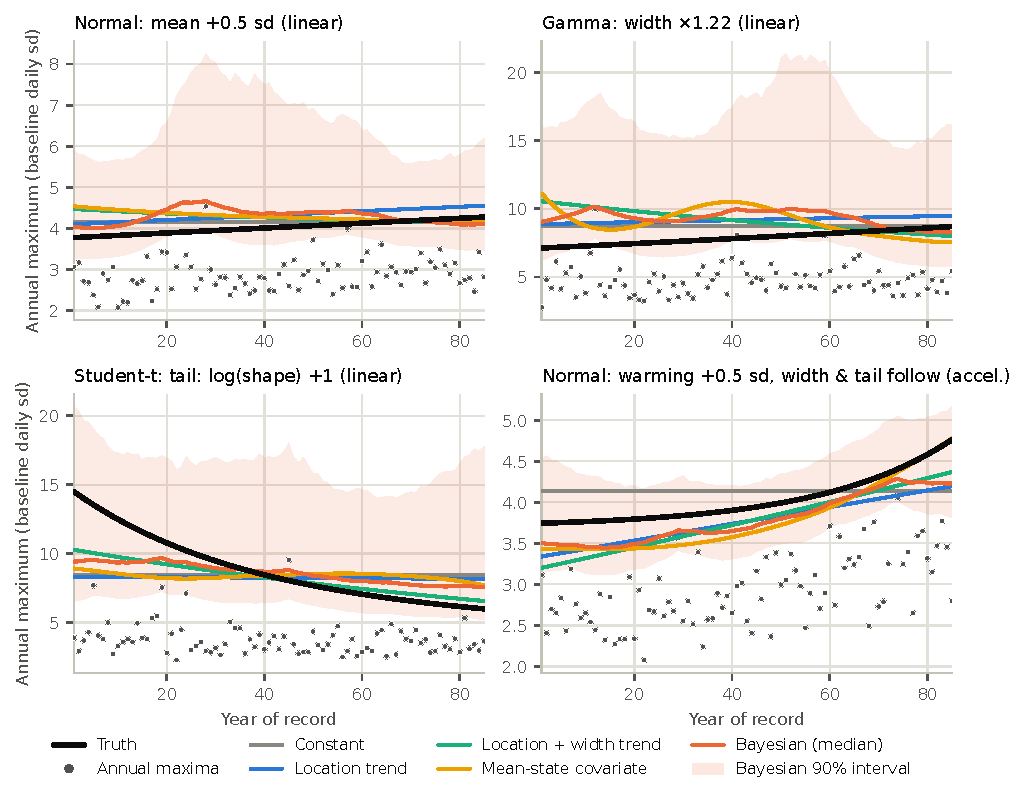
\includegraphics[width=\textwidth]{figures/fig01_examples.pdf}
\caption{Four example 85-year records (points: annual maxima), with the true 1-in-100-year level of each year (black) and six estimates of it: constant GEV (grey), location trend (blue), location + width trend (green), mean-state covariate model (yellow) and the Bayesian random-walk model's posterior median (orange), with its 90\% credible interval shaded. Titles: parent distribution and true change (accel.: accelerating). Units: baseline daily standard deviation. The 1-in-100-year level lies above almost every annual maximum, so it must be extrapolated from them.}
\label{fig:examples}
\end{figure}

\begin{figure}[H]
\centering
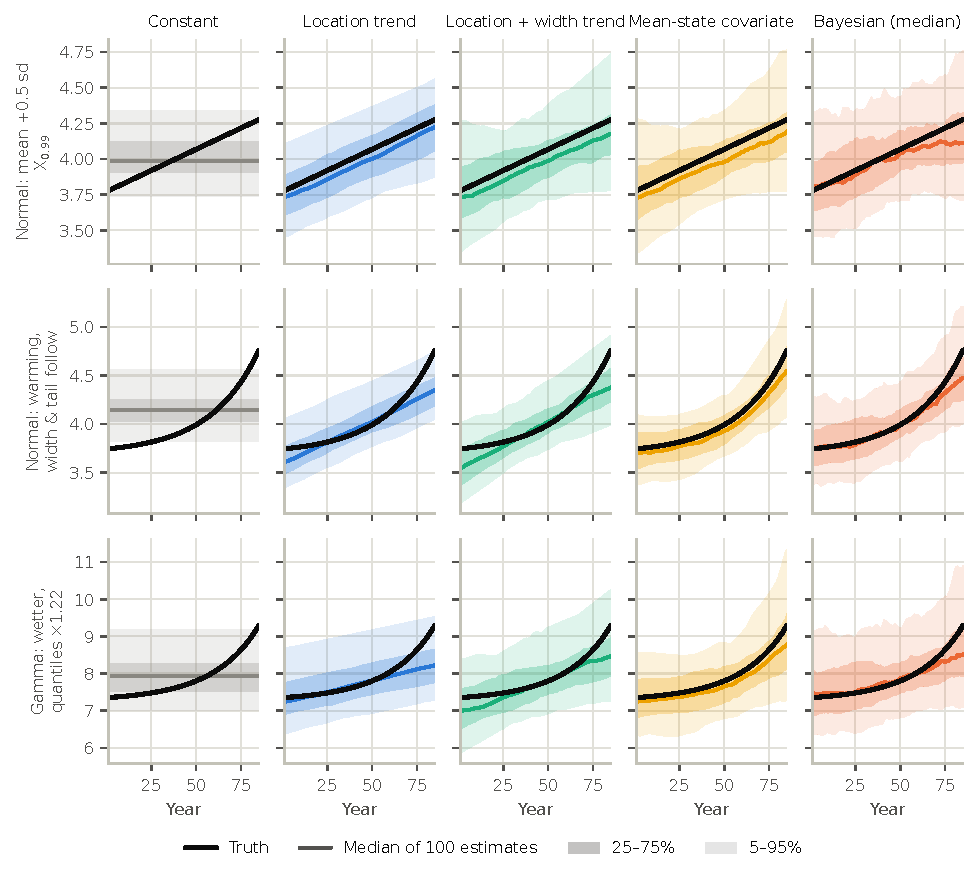
\includegraphics[width=\textwidth]{figures/fig02_spread.pdf}
\caption{How the estimated 1-in-100-year level varies across 100 synthetic 85-year records of the same climate. Columns: estimator (Bayesian: posterior median). Rows: normal parent with a linear mean rise (top); normal parent whose width and tail follow an accelerating mean (middle); gamma (precipitation-like) parent whose quantiles all scale with an accelerating mean (bottom). In each year: median of the 100 estimates (line), 25--75\% (dark band) and 5--95\% (light band); black: the truth. Units: baseline daily standard deviation. The constant model misses the change; the others track it on average, but single records scatter widely.}
\label{fig:spread}
\end{figure}

\begin{figure}[H]
\centering
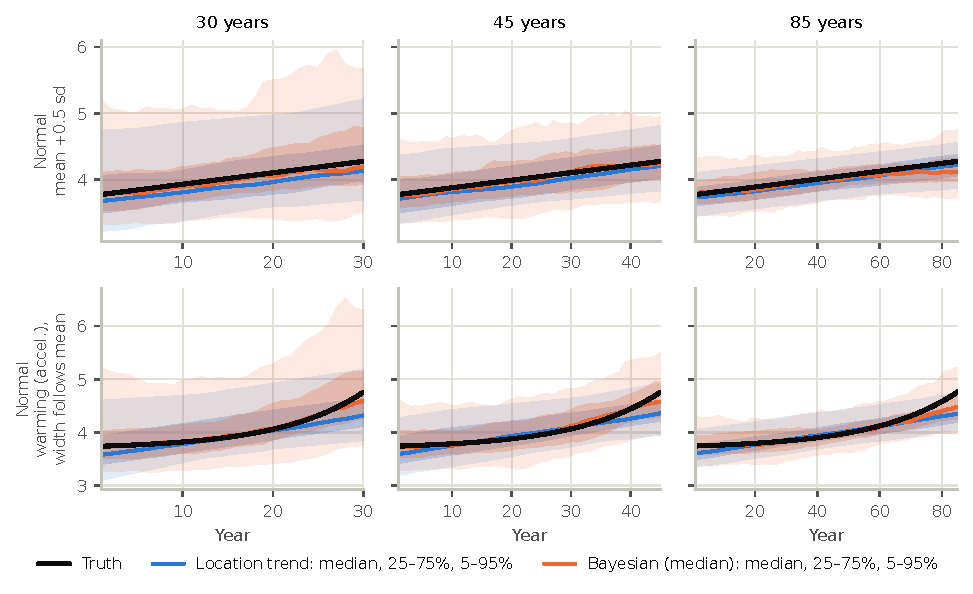
\includegraphics[width=\textwidth]{figures/fig03_record_length.pdf}
\caption{Effect of record length. Location-trend (blue) and Bayesian posterior-median (orange) estimates of the 1-in-100-year level over 100 records per panel. In each year: median of the 100 estimates (line), 25--75\% (dark band) and 5--95\% (light band); black: the truth. Columns: 30, 45 and 85 years, with the same total change in each, so the change per year is larger for shorter records. Rows: normal parent, linear mean rise of 0.5 daily sd (top) and accelerating warming with the width following the mean (bottom). Units: baseline daily standard deviation. At 30 years the spread across records is much larger than the change itself.}
\label{fig:length}
\end{figure}

\begin{figure}[H]
\centering
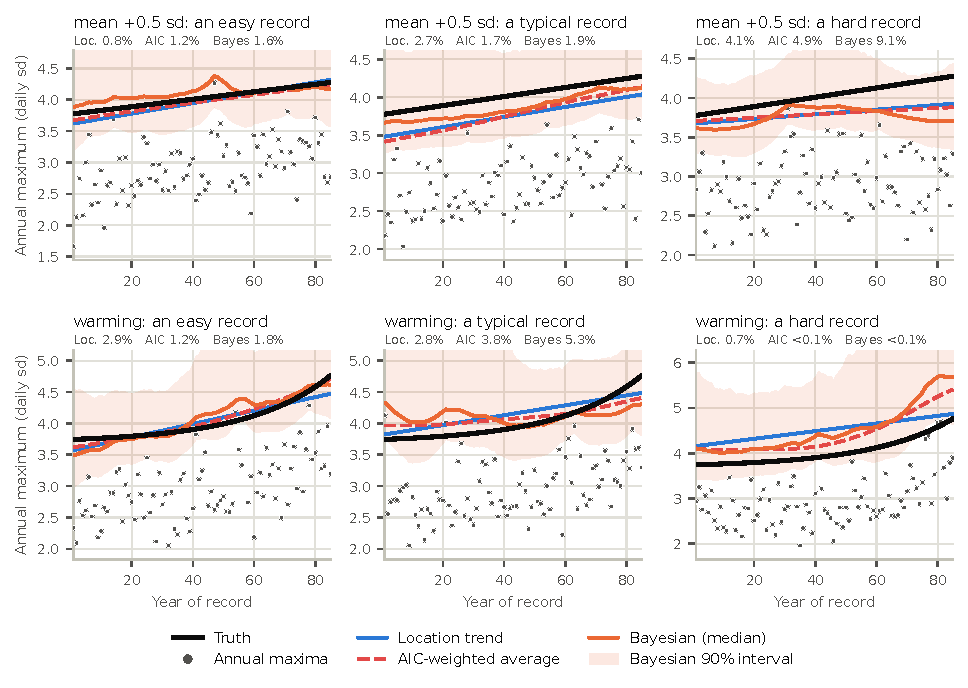
\includegraphics[width=\textwidth]{figures/fig_records_luck.pdf}
\caption{The luck of the draw: three 85-year records of the same climate, an easy, a typical and a hard one (10th, 50th and 90th percentiles of 100 records ranked by the average error of the three estimates in the last year, $|\log(\text{true exceedance}/1\%)|$). Normal parent; top: mean +0.5 daily sd, linear; bottom: accelerating warming with width and tail following the mean. Points: annual maxima; black: true 1-in-100-year level; blue: location trend; red, dashed: AIC-weighted average of four simple models; orange: Bayesian posterior median, with its 90\% credible interval shaded. Above each panel: the true probability that each estimate of the last year's level is exceeded (ideal 1\%; above 2\%: risk understated at least twofold; below 0.5\%: overstated; Loc.: location trend, AIC: AIC-weighted average, Bayes: Bayesian median). Units: baseline daily standard deviation. The same method can be nearly right or several-fold off depending only on the record.}
\label{fig:luck}
\end{figure}

\begin{figure}[H]
\centering
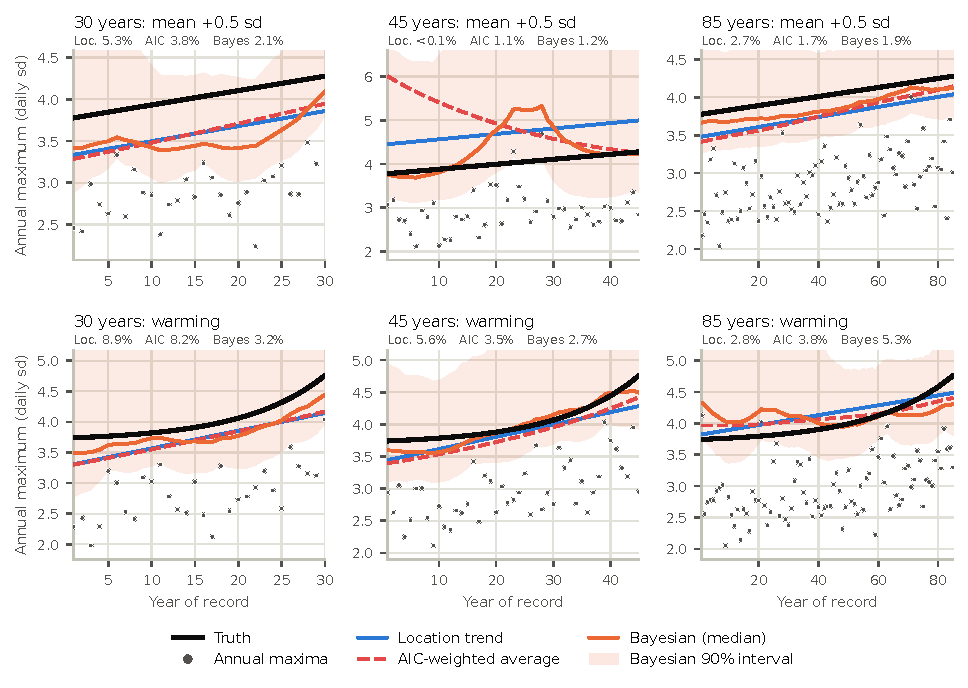
\includegraphics[width=\textwidth]{figures/fig_records_length.pdf}
\caption{Typical single records of 30, 45 and 85 years for the two cases of Figure~\ref{fig:length} (normal parent; top: mean +0.5 daily sd, linear; bottom: accelerating warming with the width following the mean). ``Typical'': the median of 100 records ranked by the average error of the three estimates in the last year, $|\log(\text{true exceedance}/1\%)|$. Points: annual maxima; black: true 1-in-100-year level; blue: location trend; red, dashed: AIC-weighted average of four simple models; orange: Bayesian posterior median, with its 90\% credible interval shaded. Above each panel: the true probability that each estimate of the last year's level is exceeded (ideal 1\%; above 2\%: risk understated at least twofold; below 0.5\%: overstated; Loc.: location trend, AIC: AIC-weighted average, Bayes: Bayesian median). Units: baseline daily standard deviation.}
\label{fig:reclength}
\end{figure}

\subsection{Single records, case by case}

Figures~\ref{fig:rnormal}--\ref{fig:rbeta} show, for every case of each parent, the typical
85-year record (chosen by the same rule as in Figure~\ref{fig:examples}) with three estimates: the
location trend, the AIC-weighted average and the Bayesian posterior median with its 90\% interval.
The line above each panel gives the true probability that each estimate of the last year's 99\%
level is exceeded (ideal 1\%). Single records show things that pooled scores hide.

\begin{itemize}
\item \textbf{Even a typical record is usually off by a factor of 2 somewhere.} In 23 of the 24
  typical records at least one of the three estimates misses the true risk by more than a factor of
  2. Over all 85-year standard records, at least one of the three misses in 75\% and all three in
  36\%.
\item \textbf{Estimates from one record err together.} They are fitted to the same few extremes, so
  a record with unusually large or small maxima pulls them all the same way: the correlation between
  their log exceedance probabilities over records is 0.56--0.76. Agreement between methods applied
  to one record is therefore weak evidence that they are right.
\item \textbf{Flexible estimates can invent a change.} In the typical no-change records for the
  gamma and $t$ parents, a few large values in the second half make the AIC-weighted average and the
  Bayesian model rise when nothing changes, so they overstate the current risk (exceedance
  0.3--0.7\%), while the location trend stays near the truth (0.9--1.2\%).
\item \textbf{A small error in level can be a large error in risk.} For the bounded beta parent the
  estimates look close to the truth, yet their exceedance probabilities range from below 0.1\% to
  nearly 4\%, because its annual maxima vary little from year to year, so the probability of
  exceeding a level changes quickly with the level.
\end{itemize}

\begin{figure}[H]
\centering
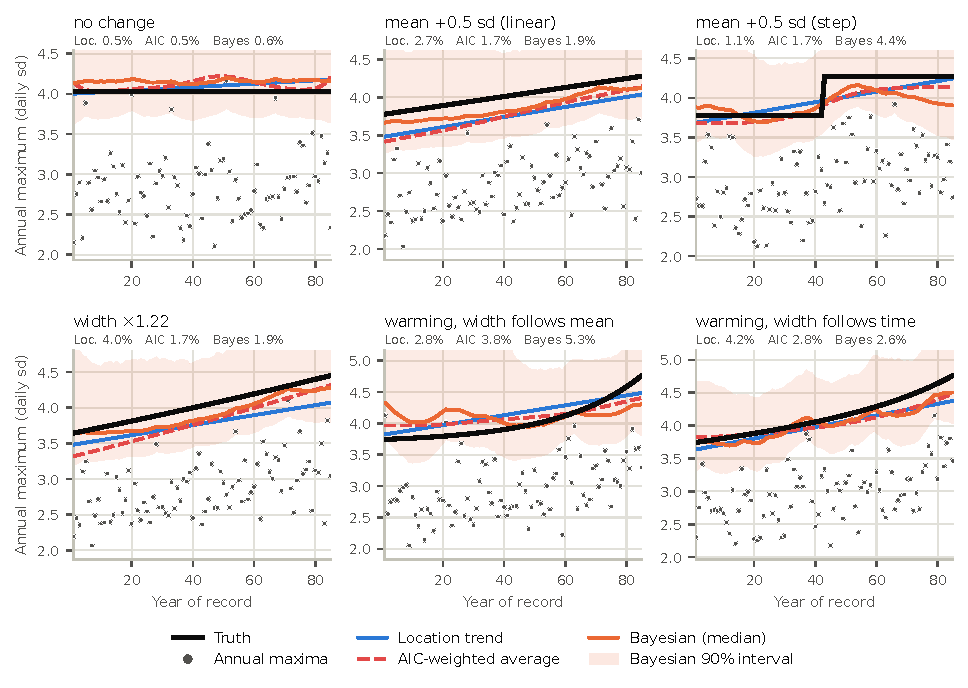
\includegraphics[width=\textwidth]{figures/fig_records_normal.pdf}
\caption{Normal (temperature-like) parent: one typical 85-year record for every case (panel titles). ``Typical'': the median of 100 records ranked by the average error of the three estimates in the last year, $|\log(\text{true exceedance}/1\%)|$. Points: annual maxima; black: true 1-in-100-year level; blue: location trend; red, dashed: AIC-weighted average of four simple models; orange: Bayesian posterior median, with its 90\% credible interval shaded. Above each panel: the true probability that each estimate of the last year's level is exceeded (ideal 1\%; above 2\%: risk understated at least twofold; below 0.5\%: overstated; Loc.: location trend, AIC: AIC-weighted average, Bayes: Bayesian median). Units: baseline daily standard deviation.}
\label{fig:rnormal}
\end{figure}
\begin{figure}[H]
\centering
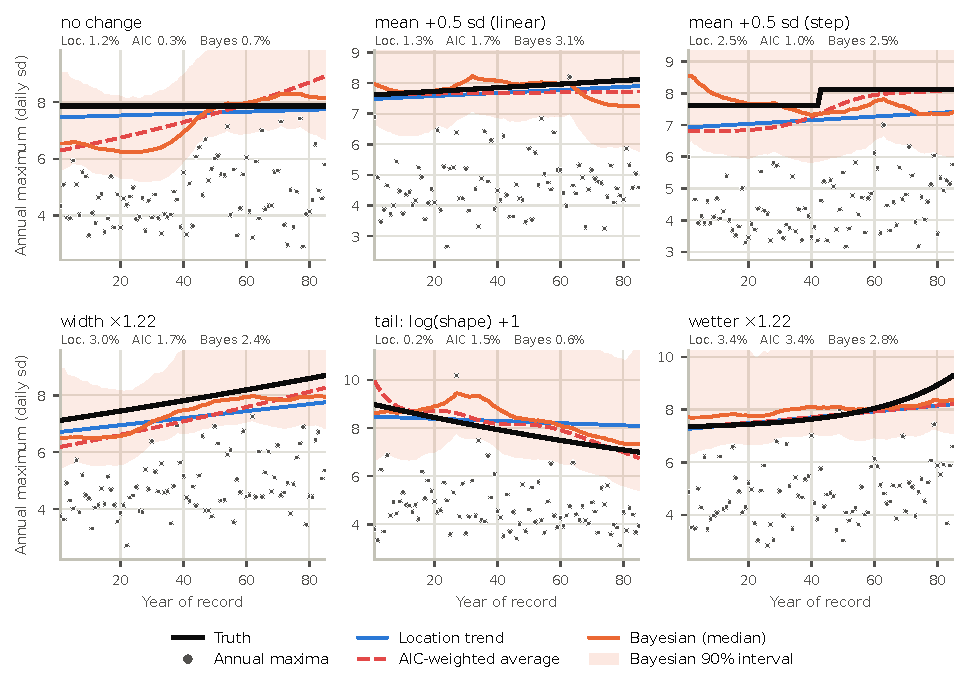
\includegraphics[width=\textwidth]{figures/fig_records_gamma.pdf}
\caption{Gamma (precipitation-like) parent: one typical 85-year record for every case (panel titles). ``Typical'': the median of 100 records ranked by the average error of the three estimates in the last year, $|\log(\text{true exceedance}/1\%)|$. Points: annual maxima; black: true 1-in-100-year level; blue: location trend; red, dashed: AIC-weighted average of four simple models; orange: Bayesian posterior median, with its 90\% credible interval shaded. Above each panel: the true probability that each estimate of the last year's level is exceeded (ideal 1\%; above 2\%: risk understated at least twofold; below 0.5\%: overstated; Loc.: location trend, AIC: AIC-weighted average, Bayes: Bayesian median). Units: baseline daily standard deviation.}
\label{fig:rgamma}
\end{figure}
\begin{figure}[H]
\centering
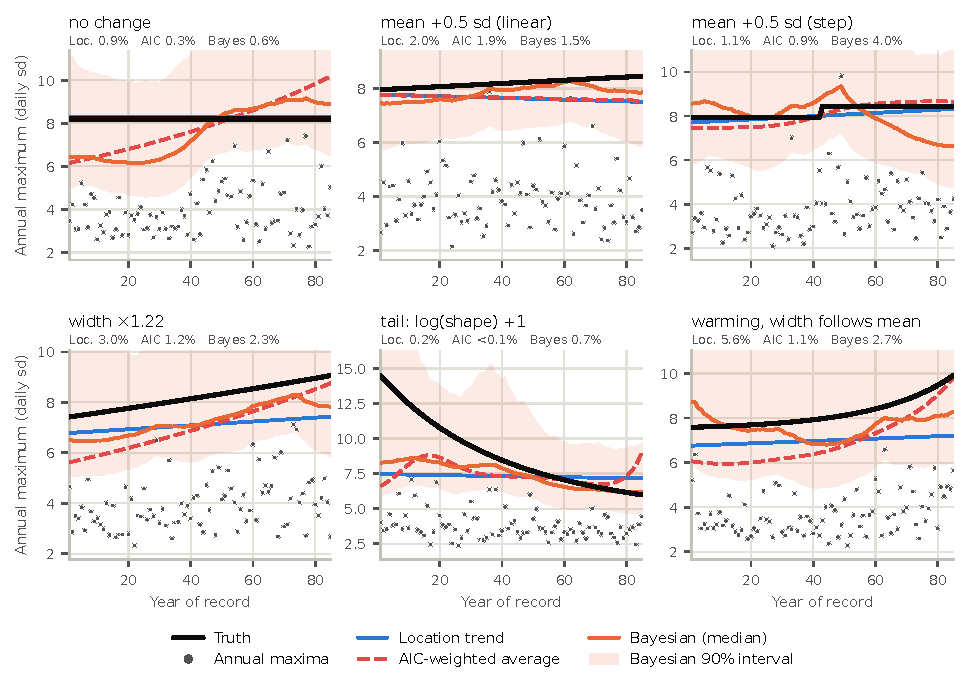
\includegraphics[width=\textwidth]{figures/fig_records_t.pdf}
\caption{Student-$t$ (heavy-tailed) parent: one typical 85-year record for every case (panel titles). ``Typical'': the median of 100 records ranked by the average error of the three estimates in the last year, $|\log(\text{true exceedance}/1\%)|$. Points: annual maxima; black: true 1-in-100-year level; blue: location trend; red, dashed: AIC-weighted average of four simple models; orange: Bayesian posterior median, with its 90\% credible interval shaded. Above each panel: the true probability that each estimate of the last year's level is exceeded (ideal 1\%; above 2\%: risk understated at least twofold; below 0.5\%: overstated; Loc.: location trend, AIC: AIC-weighted average, Bayes: Bayesian median). Units: baseline daily standard deviation.}
\label{fig:rt}
\end{figure}
\begin{figure}[H]
\centering
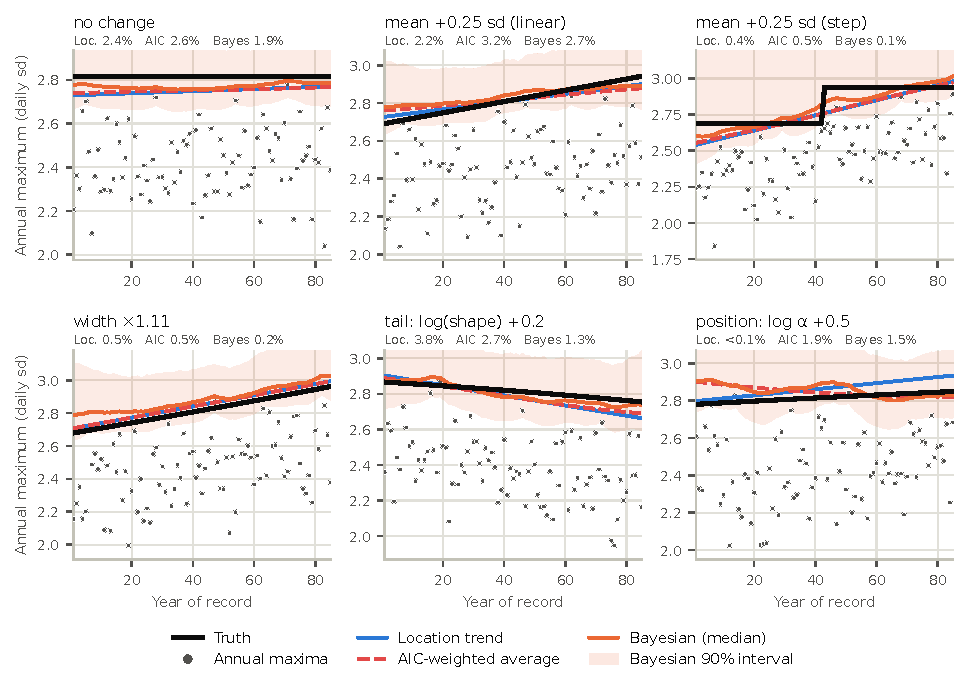
\includegraphics[width=\textwidth]{figures/fig_records_beta.pdf}
\caption{Beta (bounded) parent: one typical 85-year record for every case (panel titles). ``Typical'': the median of 100 records ranked by the average error of the three estimates in the last year, $|\log(\text{true exceedance}/1\%)|$. Points: annual maxima; black: true 1-in-100-year level; blue: location trend; red, dashed: AIC-weighted average of four simple models; orange: Bayesian posterior median, with its 90\% credible interval shaded. Above each panel: the true probability that each estimate of the last year's level is exceeded (ideal 1\%; above 2\%: risk understated at least twofold; below 0.5\%: overstated; Loc.: location trend, AIC: AIC-weighted average, Bayes: Bayesian median). Units: baseline daily standard deviation.}
\label{fig:rbeta}
\end{figure}

\subsection{Spread over records, case by case}

Figures~\ref{fig:pnormal}--\ref{fig:pbeta} repeat Figure~\ref{fig:length} for every standard
case, one figure per parent, comparing the location trend (blue) with the Bayesian posterior median
(orange). Four patterns recur.

\begin{itemize}
\item \textbf{Mean and width changes are tracked on average by both estimators}, in all four
  parents. What changes with record length is the spread: the 5--95\% band at 85 years is 37--50\% as
  wide as at 30 years.
\item \textbf{A step change is smoothed into a ramp.} Neither estimator locates the step; the
  location trend replaces it by a straight line, and the Bayesian median by a gentler rise.
\item \textbf{Short records from skewed or heavy-tailed parents give the Bayesian model a long
  upper tail.} At 30 years the upper edge of its 5--95\% band for the gamma and $t$ parents lies far
  above the truth (up to about 2.5 times the true level for the $t$), because the posterior of the tail
  index is wide and right-skewed when there are few maxima.
\item \textbf{Tail changes are where the two estimators differ most.} The location trend cannot
  represent a change in tail: it captures about a third of the fall in the 99\% level for the
  gamma parent and almost none (5--7\%) for the $t$. The Bayesian median captures more, 51--64\%
  for the gamma and 37--50\% for the $t$, increasing with record length. In the bounded beta parent the location trend does the opposite and overshoots the tail
  and position changes (by a factor of about 1.9 for the tail change), presumably because a straight-line location with fixed scale and shape is
  the only way it can absorb a change in the shape of the maxima near the bound.
\end{itemize}

\begin{figure}[H]
\centering
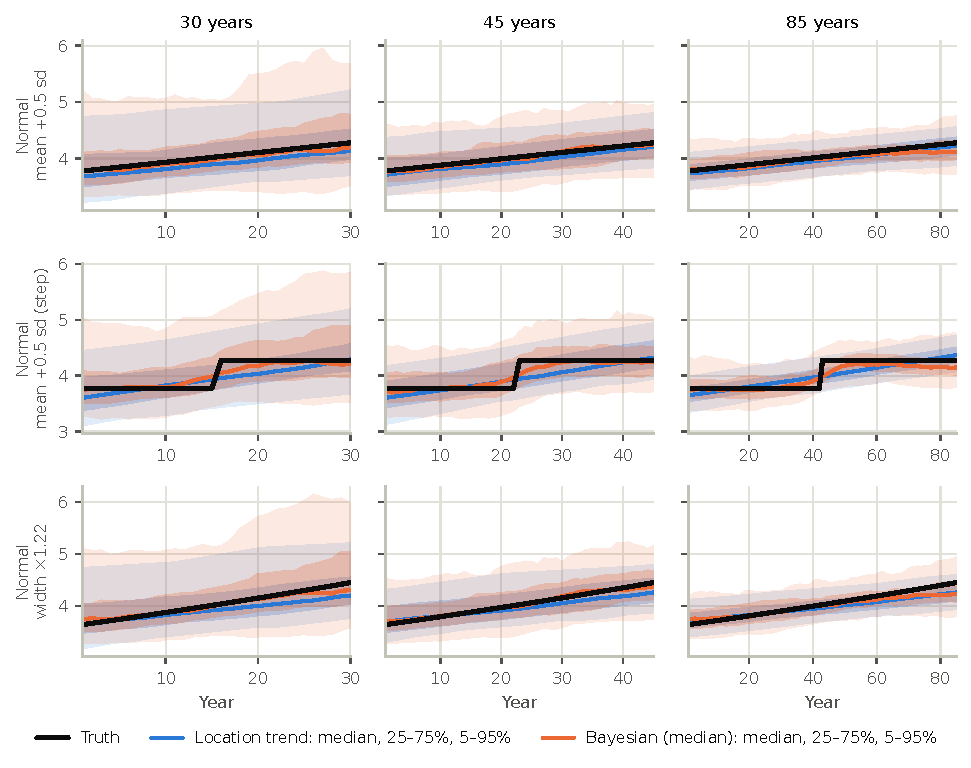
\includegraphics[width=\textwidth,height=0.78\textheight,keepaspectratio]{figures/fig_paths_normal.pdf}
\caption{Normal (temperature-like) parent: how the estimated 1-in-100-year level varies across 100 synthetic records of the same climate, for each standard change (rows) and record length (columns; the total change over the record is the same in each column). Blue: location trend; orange: Bayesian posterior median. In each year: median of the 100 estimates (line), 25--75\% (dark band) and 5--95\% (light band); black: the truth. Units: baseline daily standard deviation.}
\label{fig:pnormal}
\end{figure}
\begin{figure}[H]
\centering
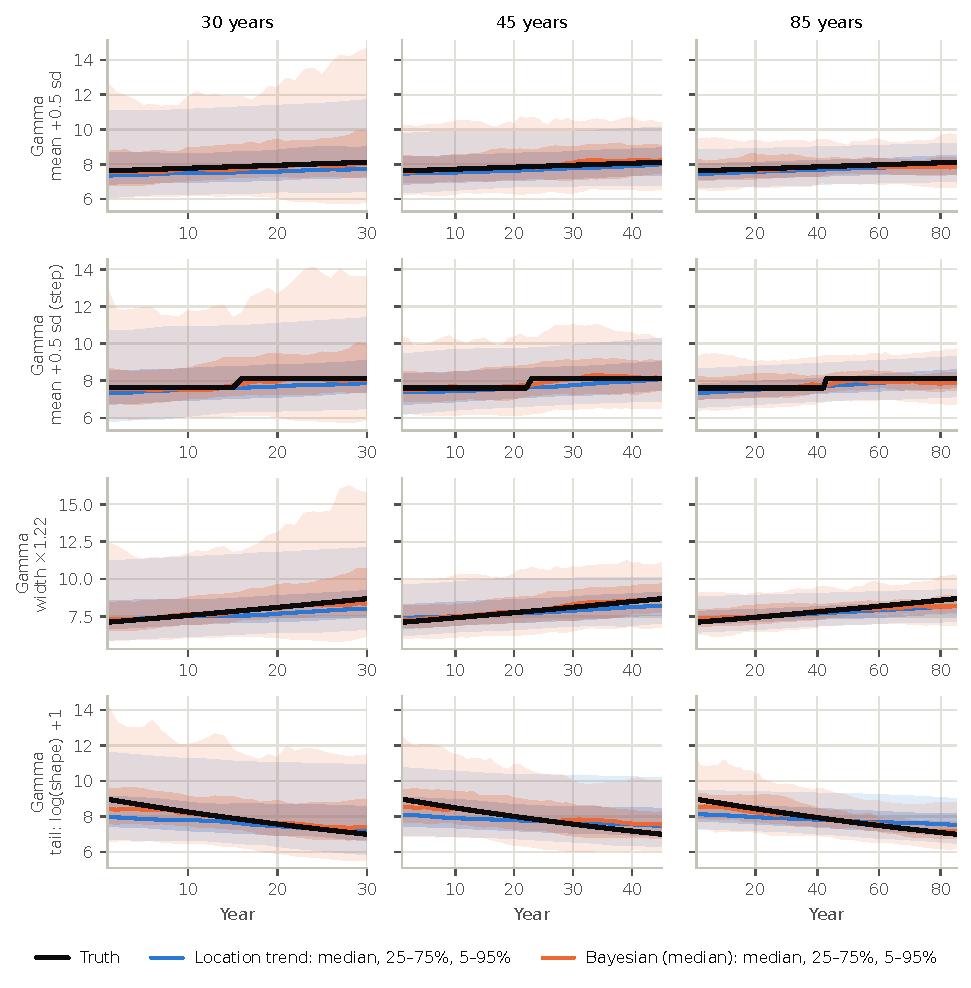
\includegraphics[width=\textwidth,height=0.78\textheight,keepaspectratio]{figures/fig_paths_gamma.pdf}
\caption{Gamma (precipitation-like) parent: how the estimated 1-in-100-year level varies across 100 synthetic records of the same climate, for each standard change (rows) and record length (columns; the total change over the record is the same in each column). Blue: location trend; orange: Bayesian posterior median. In each year: median of the 100 estimates (line), 25--75\% (dark band) and 5--95\% (light band); black: the truth. Units: baseline daily standard deviation.}
\label{fig:pgamma}
\end{figure}
\begin{figure}[H]
\centering
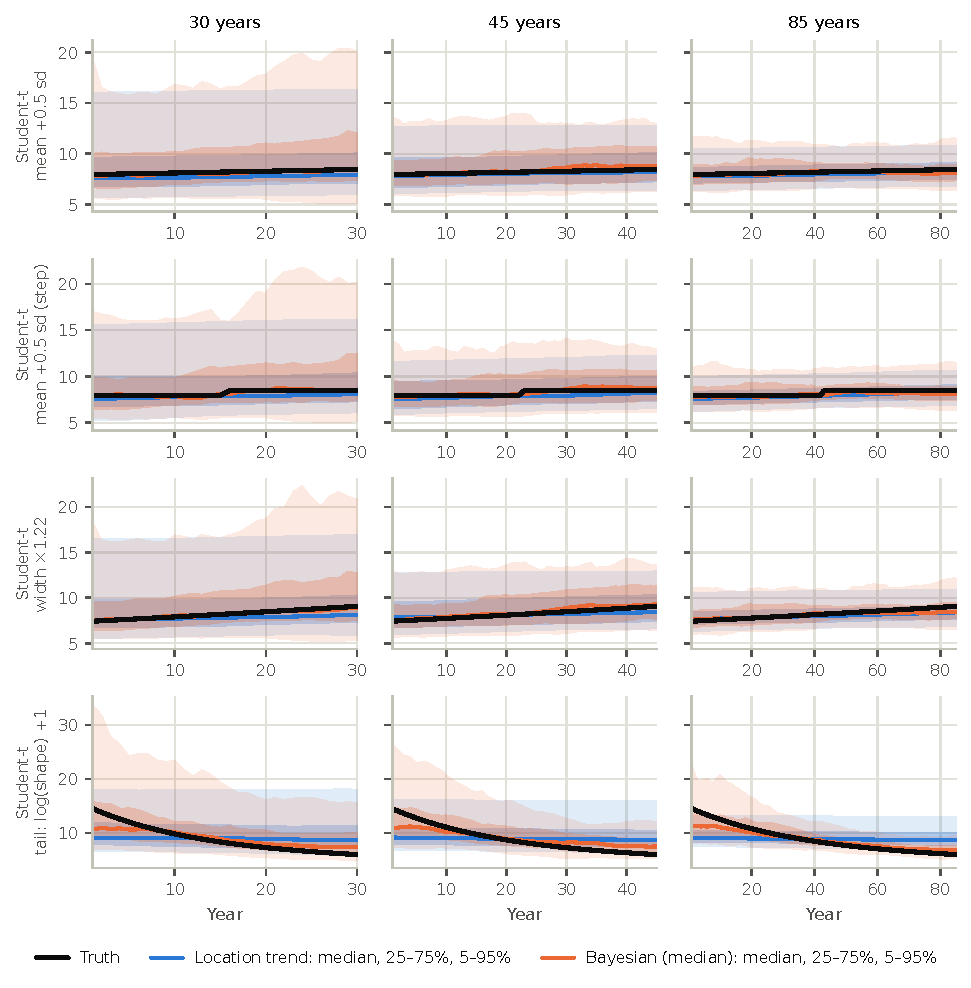
\includegraphics[width=\textwidth,height=0.78\textheight,keepaspectratio]{figures/fig_paths_t.pdf}
\caption{Student-$t$ (heavy-tailed) parent: how the estimated 1-in-100-year level varies across 100 synthetic records of the same climate, for each standard change (rows) and record length (columns; the total change over the record is the same in each column). Blue: location trend; orange: Bayesian posterior median. In each year: median of the 100 estimates (line), 25--75\% (dark band) and 5--95\% (light band); black: the truth. Units: baseline daily standard deviation.}
\label{fig:pt}
\end{figure}
\begin{figure}[H]
\centering
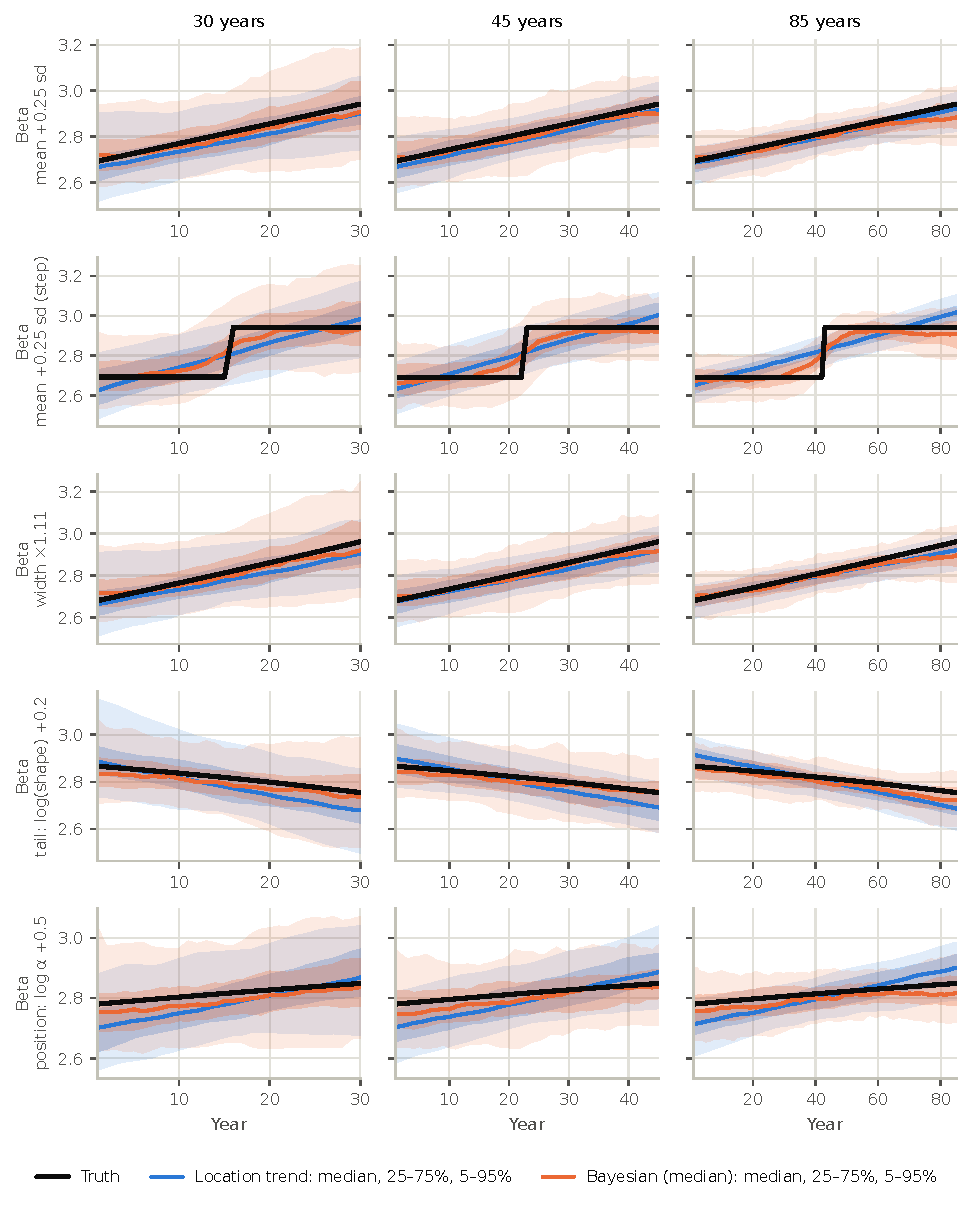
\includegraphics[width=\textwidth,height=0.78\textheight,keepaspectratio]{figures/fig_paths_beta.pdf}
\caption{Beta (bounded) parent: how the estimated 1-in-100-year level varies across 100 synthetic records of the same climate, for each standard change (rows) and record length (columns; the total change over the record is the same in each column). Blue: location trend; orange: Bayesian posterior median. In each year: median of the 100 estimates (line), 25--75\% (dark band) and 5--95\% (light band); black: the truth. Units: baseline daily standard deviation.}
\label{fig:pbeta}
\end{figure}

\subsection{The noise floor}

Much of the error has nothing to do with change. With no change and the correctly specified
constant model, the estimated $\Xp$ misses the risk by more than a factor of 2 in 44\% of 85-year
records: it understates it at least twofold in 27\% and overstates it at least twofold in 18\%. For
45-year records 68\% miss (38\% and 30\%), and for 30-year records 71\% (44\% and 27\%). The median exceedance probability is 1.3\% rather than
1\%: the sampling distribution of an estimated high quantile is skewed, so the typical estimate
is a little low. This floor is the yardstick for the results below. An estimator that allows for
change should not be expected to beat it, and it pays for its flexibility with extra variance when
the change is small.

\subsection{Accuracy of the current 99\% level}

Figures~\ref{fig:exceedance} and \ref{fig:heatmap} and Table~\ref{tab:headline} pool the results
over the standard cases (20 cases including the four with no change) and the covariate-model cases
(7 cases).

\begin{itemize}
\item \textbf{Estimators differ as much in the direction of their errors as in how often they
  miss.} At 85 years the location trend understates the risk twofold in 30\% of records and
  overstates it in 26\%; the Bayesian median understates in 39\% and overstates in 20\%. The
  Bayesian posterior mean is the extreme case: it rarely understates (20\%) but overstates in 51\%.
  Below we rank by the total and give the split; Table~\ref{tab:headline} has both for every
  estimator.
\item \textbf{At 85 years an average of simple models does best} over the standard cases: the
  AIC-weighted average of the constant, location-trend, location + width and covariate models misses
  51\% of records (30\% understated, 20\% overstated), $5.5\pm1.0$ points fewer than the location trend
  or the location + width trend (both 56\%). Ignoring change (constant, 65\%) or using only the last
  30 years (65\%) is much worse, and trends in all three parameters (70\%) pay for their flexibility
  with extra variance.
\item \textbf{The Bayesian model is about as accurate as the simple trends}: it misses 75\%, 70\% and
  59\% of records at 30, 45 and 85 years, against 73\%, 69\% and 56\% for the location trend (paired
  differences of 1--3 points, $\pm1.2$). Its errors lean toward overstatement at 30 years (39\%
  overstated against 33\%) and toward understatement at 85 years (39\% understated against 30\%).
  Its posterior mean is a poor point estimate: the posterior of a high quantile is right-skewed, so
  the mean overstates the level (median exceedance 0.5\% at 85 years, and below 0.01\% at 30 years,
  where the posterior has a very long right tail).
\item \textbf{With 30 or 45 years the method hardly matters}: the location trend, location + width
  trend, covariate model, AIC choices and Bayesian model miss 73--76\% of 30-year and 68--72\% of
  45-year records, against no-change floors of 71\% and 68\%.
\item \textbf{Three values per year help} when declustered: at 85 years the AIC-weighted average
  misses 44\% and the location + width trend 45\% (from 51\% and 56\%), the location trend 51\% and
  the Bayesian model 53\%. For the trend models and the average both kinds of miss fall; the
  Bayesian model gains on understatement only. Figure~\ref{fig:pk} shows the
  bands narrowing a little, and the Bayesian median following the $t$ tail change more closely; it
  also shows the unconverged Bayesian fits for the beta parent (Section~\ref{sec:bayes}) as a wide
  upper band early in the 85-year record.
\item \textbf{Record length matters more than the method.} Every estimator is worse at 30 years
  than at 85, and the spread between these methods (3--4 points at 30 and 45 years, 8 at 85) is
  much smaller than the floor itself.
\end{itemize}

\begin{figure}[H]
\centering
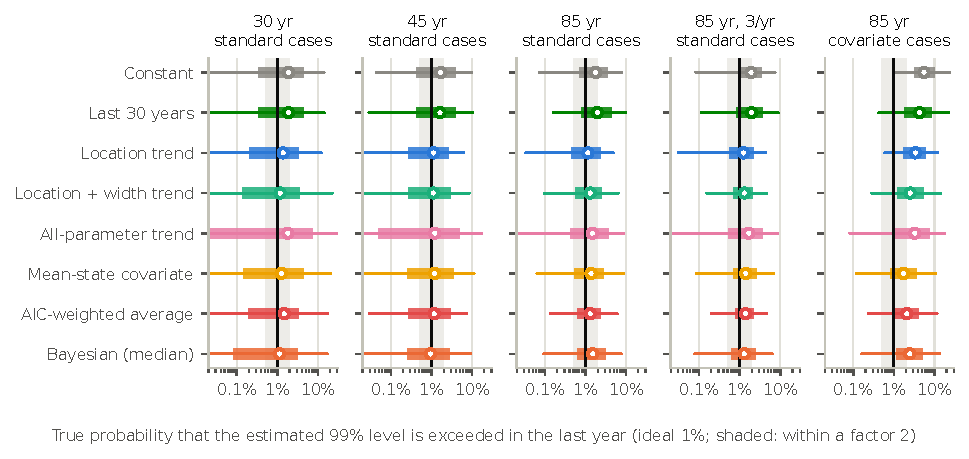
\includegraphics[width=\textwidth]{figures/fig06_exceedance.pdf}
\caption{Accuracy of the estimated 1-in-100-year level in the last year of the record, for eight estimators (rows). Plotted: the true probability that the last year's annual maximum exceeds the estimate. An ideal estimate gives 1\% (vertical line); left of it the level is too high (risk overstated), right of it too low (understated). Shaded: within a factor of 2 of 1\%. Over all records of a panel: white circle, median; thick bar, 25--75\%; thin line, 5--95\%. Panels: record length and set of cases (3/yr: three values per year instead of the annual maximum). Standard cases: the four parent distributions with no change or a linear or step change in their mean, width or tail. Covariate-model cases: the width (and for some parents the tail) follows an accelerating mean state; for the gamma, every quantile scales with the mean. Most medians are near 1\%, but single records range over one to more than two orders of magnitude.}
\label{fig:exceedance}
\end{figure}

\begin{figure}[H]
\centering
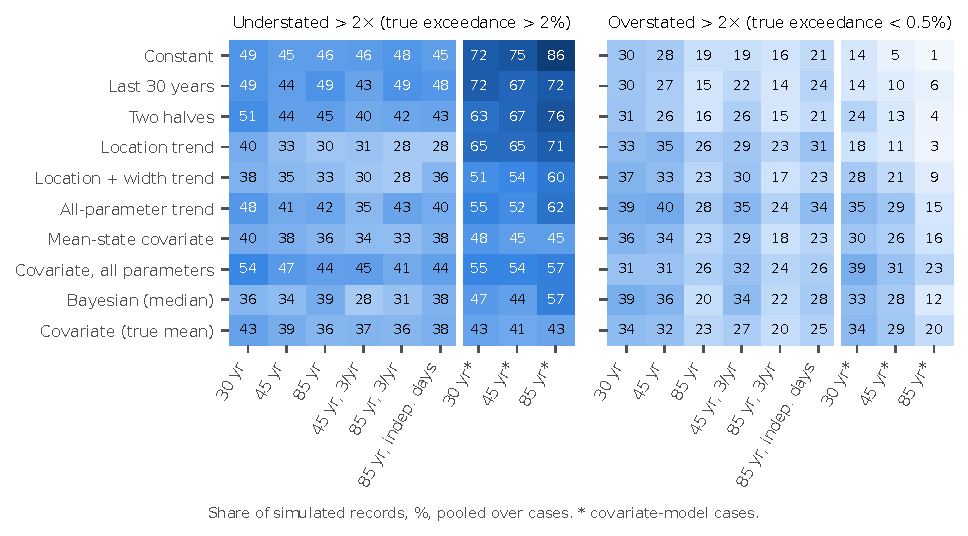
\includegraphics[width=\textwidth]{figures/fig07_heatmap.pdf}
\caption{Share of records (\%) in which the estimated 1-in-100-year level of the last year is off by more than a factor of 2 in its risk. Left: missed either way; middle: risk understated (true probability of exceeding the estimate above 2\%: the level is too low); right: risk overstated (below 0.5\%: the level is too high). Missed = understated + overstated. Rows: estimators. Columns: record length in years (3/yr: three values per year), for the standard and, separately, the covariate-model cases. Darker: larger share. Standard cases: the four parent distributions with no change or a linear or step change in their mean, width or tail. Covariate-model cases: the width (and for some parents the tail) follows an accelerating mean state; for the gamma, every quantile scales with the mean. Even the best estimators miss about half of 85-year records and three-quarters of 30-year records.}
\label{fig:heatmap}
\end{figure}

\begin{figure}[H]
\centering
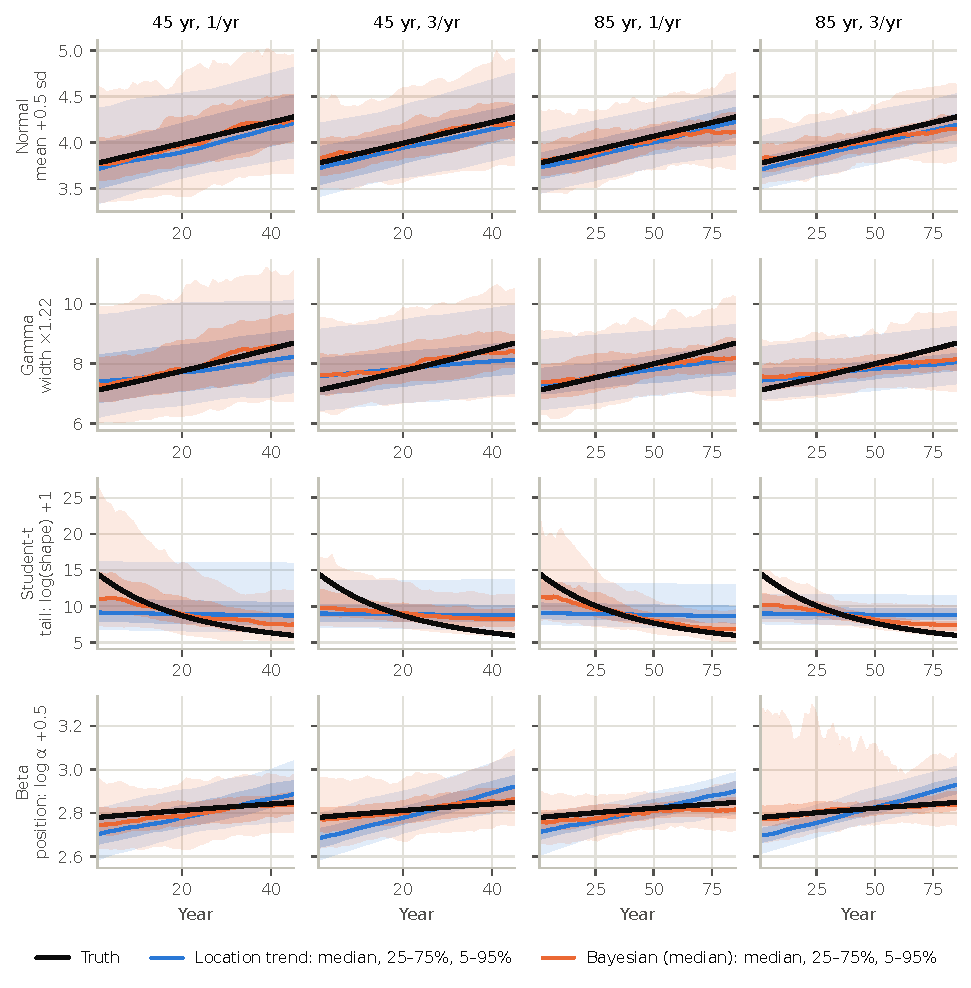
\includegraphics[width=\textwidth]{figures/fig_paths_values_per_year.pdf}
\caption{One value per year (the annual maximum) against three (the three largest, at least 3 days apart), at 45 and 85 years (columns), for four cases (rows: normal, mean +0.5 daily sd; gamma, width $\times$1.22; Student-$t$, tail lightened, log of degrees of freedom +1; beta, position change). Blue: location trend; orange: Bayesian posterior median. In each year: median of the 100 estimates (line), 25--75\% (dark band) and 5--95\% (light band); black: the truth. Units: baseline daily standard deviation. Three values per year generally narrow the bands.}
\label{fig:pk}
\end{figure}

\begin{table}[H]
\centering
\scriptsize
\setlength{\tabcolsep}{2.3pt}
\begin{tabular}{lrrrrrrrrrrrrrrrr}
\toprule
 & \multicolumn{4}{c}{30 yr} & \multicolumn{4}{c}{45 yr} & \multicolumn{4}{c}{85 yr} & \multicolumn{4}{c}{85 yr, 3/yr} \\
\cmidrule(lr){2-5} \cmidrule(lr){6-9} \cmidrule(lr){10-13} \cmidrule(lr){14-17}
Estimator & med. & miss & $>$2\% & $<$0.5\% & med. & miss & $>$2\% & $<$0.5\% & med. & miss & $>$2\% & $<$0.5\% & med. & miss & $>$2\% & $<$0.5\% \\
\midrule
\multicolumn{17}{l}{\emph{Standard cases}} \\
Constant & 1.88 & \textbf{78} & 49 & 30 & 1.69 & \textbf{73} & 45 & 28 & 1.77 & \textbf{65} & 46 & 19 & 1.91 & \textbf{64} & 48 & 16 \\
Last 30 years & 1.88 & \textbf{78} & 49 & 30 & 1.62 & \textbf{71} & 44 & 27 & 1.94 & \textbf{65} & 49 & 15 & 1.96 & \textbf{63} & 49 & 14 \\
Two halves & 2.07 & \textbf{82} & 51 & 31 & 1.67 & \textbf{70} & 44 & 26 & 1.75 & \textbf{61} & 45 & 16 & 1.68 & \textbf{57} & 42 & 15 \\
Location trend & 1.39 & \textbf{73} & 40 & 33 & 1.13 & \textbf{69} & 33 & 35 & 1.14 & \textbf{56} & 30 & 26 & 1.24 & \textbf{51} & 28 & 23 \\
Loc. + width trend & 1.17 & \textbf{75} & 38 & 37 & 1.12 & \textbf{68} & 35 & 33 & 1.30 & \textbf{56} & 33 & 23 & 1.31 & \textbf{45} & 28 & 17 \\
All-param. trend & 1.81 & \textbf{86} & 48 & 39 & 1.21 & \textbf{81} & 41 & 40 & 1.47 & \textbf{70} & 42 & 28 & 1.68 & \textbf{67} & 43 & 24 \\
Mean-state cov. & 1.26 & \textbf{76} & 40 & 36 & 1.20 & \textbf{72} & 38 & 34 & 1.37 & \textbf{59} & 36 & 23 & 1.41 & \textbf{51} & 33 & 18 \\
Cov., all param. & 2.57 & \textbf{85} & 54 & 31 & 1.75 & \textbf{78} & 47 & 31 & 1.64 & \textbf{70} & 44 & 26 & 1.51 & \textbf{64} & 41 & 24 \\
Data-chosen (AIC) & 1.48 & \textbf{76} & 42 & 33 & 1.27 & \textbf{71} & 38 & 33 & 1.31 & \textbf{55} & 34 & 21 & 1.38 & \textbf{45} & 30 & 16 \\
AIC-weighted avg. & 1.47 & \textbf{75} & 41 & 34 & 1.17 & \textbf{69} & 36 & 33 & 1.30 & \textbf{51} & 30 & 20 & 1.40 & \textbf{44} & 28 & 15 \\
Bayes (median) & 1.13 & \textbf{75} & 36 & 39 & 0.94 & \textbf{70} & 34 & 36 & 1.50 & \textbf{59} & 39 & 20 & 1.30 & \textbf{53} & 31 & 22 \\
Bayes (mean) & 0.00 & \textbf{92} & 5 & 87 & 0.01 & \textbf{88} & 10 & 78 & 0.48 & \textbf{71} & 20 & 51 & 0.79 & \textbf{60} & 22 & 38 \\
Cov., true mean & 1.56 & \textbf{77} & 43 & 34 & 1.31 & \textbf{71} & 39 & 32 & 1.43 & \textbf{59} & 36 & 23 & 1.48 & \textbf{55} & 36 & 20 \\
Cov., all, true mean & 1.63 & \textbf{80} & 45 & 35 & 1.38 & \textbf{74} & 41 & 33 & 1.48 & \textbf{64} & 40 & 25 & 1.57 & \textbf{61} & 39 & 22 \\
\multicolumn{17}{l}{\emph{Covariate-model cases}} \\
Constant & 5.49 & \textbf{86} & 72 & 14 & 5.34 & \textbf{80} & 75 & 5 & 5.56 & \textbf{87} & 86 & 1 &  &  &  &  \\
Last 30 years & 5.49 & \textbf{86} & 72 & 14 & 4.14 & \textbf{77} & 67 & 10 & 4.32 & \textbf{78} & 72 & 6 &  &  &  &  \\
Two halves & 4.17 & \textbf{87} & 63 & 24 & 4.15 & \textbf{80} & 67 & 13 & 4.42 & \textbf{80} & 76 & 4 &  &  &  &  \\
Location trend & 3.58 & \textbf{83} & 65 & 18 & 3.19 & \textbf{76} & 65 & 11 & 3.42 & \textbf{74} & 71 & 3 &  &  &  &  \\
Loc. + width trend & 2.20 & \textbf{79} & 51 & 28 & 2.32 & \textbf{75} & 54 & 21 & 2.53 & \textbf{69} & 60 & 9 &  &  &  &  \\
All-param. trend & 2.94 & \textbf{90} & 55 & 35 & 2.25 & \textbf{81} & 52 & 29 & 3.28 & \textbf{77} & 62 & 15 &  &  &  &  \\
Mean-state cov. & 1.85 & \textbf{78} & 48 & 30 & 1.65 & \textbf{71} & 45 & 26 & 1.73 & \textbf{62} & 45 & 16 &  &  &  &  \\
Cov., all param. & 3.72 & \textbf{93} & 55 & 39 & 2.65 & \textbf{85} & 54 & 31 & 2.83 & \textbf{80} & 57 & 23 &  &  &  &  \\
Data-chosen (AIC) & 2.68 & \textbf{82} & 57 & 25 & 2.18 & \textbf{74} & 53 & 21 & 2.04 & \textbf{63} & 50 & 12 &  &  &  &  \\
AIC-weighted avg. & 2.45 & \textbf{82} & 56 & 26 & 2.20 & \textbf{73} & 52 & 21 & 2.09 & \textbf{64} & 52 & 12 &  &  &  &  \\
Bayes (median) & 1.67 & \textbf{80} & 47 & 33 & 1.67 & \textbf{72} & 44 & 28 & 2.46 & \textbf{69} & 57 & 12 &  &  &  &  \\
Bayes (mean) & 0.00 & \textbf{94} & 5 & 89 & 0.01 & \textbf{89} & 12 & 77 & 0.69 & \textbf{72} & 28 & 45 &  &  &  &  \\
Cov., true mean & 1.40 & \textbf{77} & 43 & 34 & 1.39 & \textbf{70} & 41 & 29 & 1.61 & \textbf{63} & 43 & 20 &  &  &  &  \\
Cov., all, true mean & 2.23 & \textbf{88} & 52 & 36 & 1.46 & \textbf{85} & 46 & 39 & 2.01 & \textbf{79} & 50 & 29 &  &  &  &  \\
\bottomrule
\end{tabular}

\caption{Accuracy of each estimator's 1-in-100-year level for the last year of the record. For each design (30, 45 and 85 years; 85 yr, 3/yr: three values per year): med., the median over records of the true probability (\%) that the last year's annual maximum exceeds the estimate (ideal 1); miss (bold), the share of records (\%) in which that probability is off by more than a factor of 2 either way; $>$2\%, the share with the risk understated (estimate too low); $<$0.5\%, the share with the risk overstated (estimate too high). Miss = $>$2\% + $<$0.5\%. Standard cases: the four parent distributions with no change or a linear or step change in their mean, width or tail. Covariate-model cases: the width (and for some parents the tail) follows an accelerating mean state; for the gamma, every quantile scales with the mean. Bayes (median) and (mean): posterior median and mean of the draws' levels. Cov., true mean: oracle covariate models given the true mean.}
\label{tab:headline}
\end{table}

\subsection{Estimating the size of the change}

Figure~\ref{fig:change} shows the estimated change in $\Xp$ from the first year to the last for
every case. The location trend is precise but estimates only the part of the change that is a
shift in location: it captures between a third and four-fifths of a width change (depending on the
parent) and a third or less of a tail change in the gamma and $t$ parents. The location + width
trend and the covariate model are roughly unbiased where their form is right, but their 10--90\%
ranges are as wide as the change itself. The Bayesian model systematically shrinks the change
toward zero, most visibly for the large tail change in the $t$ parent and for the
precipitation-like cases. For a normal parent with 85 years and a true change of 0.5, the
location trend's 10--90\% range is 0.33--0.65. The location + width trend and the covariate model
span about 0 to 0.9, so even the sign is wrong in about one record in ten. The Bayesian median
change is 0.32, against the true 0.5.

\begin{figure}[H]
\centering
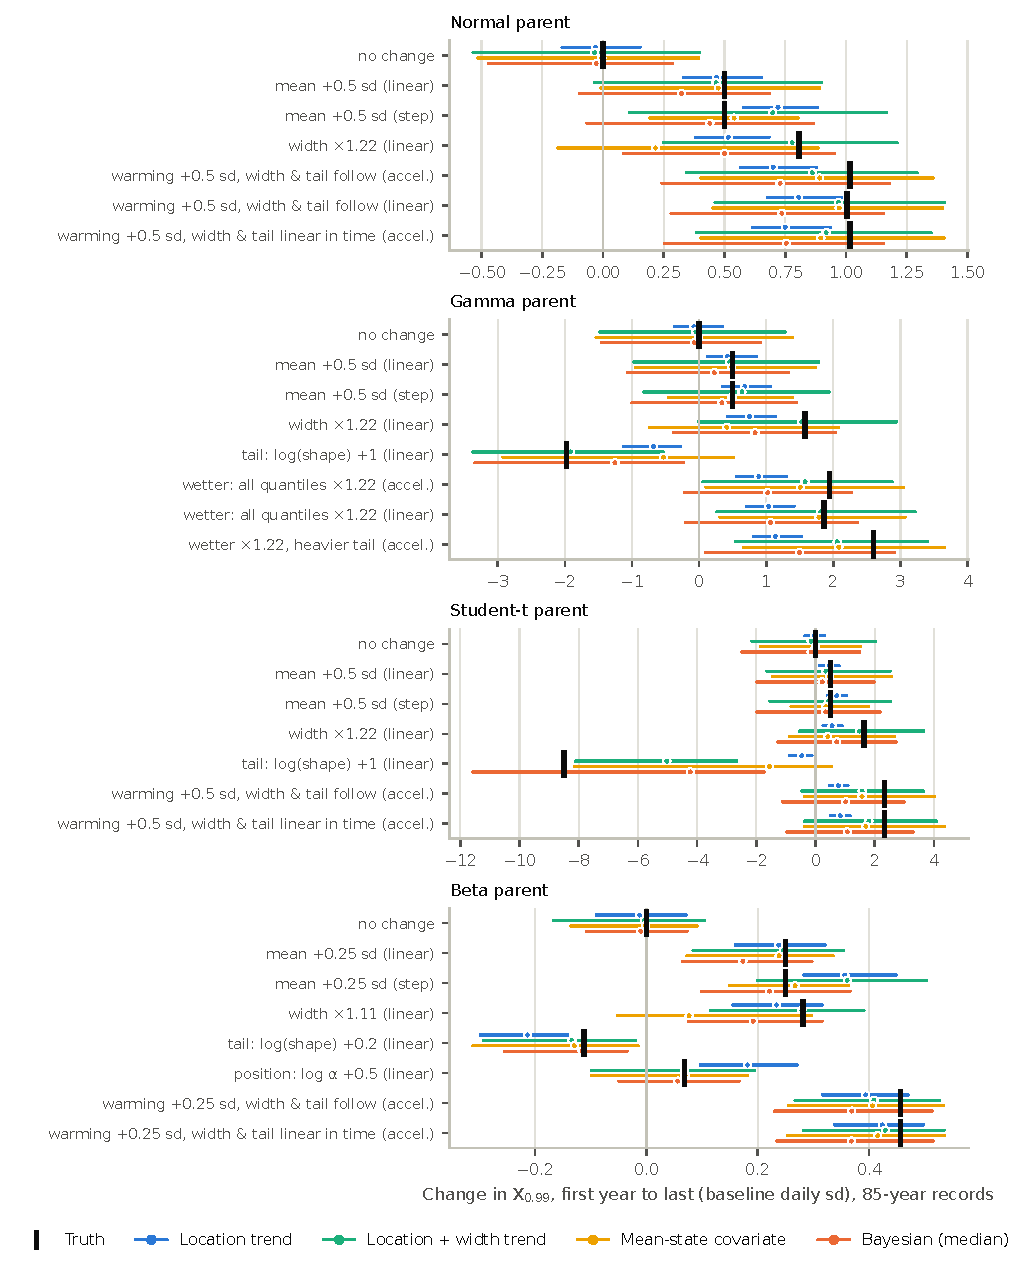
\includegraphics[width=\textwidth,height=0.78\textheight,keepaspectratio]{figures/fig08_change.pdf}
\caption{Estimated change in the 1-in-100-year level from the first to the last year of 85-year records, for every case (rows, grouped by parent), against the true change (black bar). Dots: median over 100 records; lines: 10--90\%. Location trend (blue), location + width trend (green), mean-state covariate (yellow), Bayesian posterior median (orange). Units: baseline daily standard deviation. The spread across records is often as large as the change, and the Bayesian model shrinks changes toward zero.}
\label{fig:change}
\end{figure}

%=====================================================================================
\section{Using the wrong model}\label{sec:wrong}

A change in extremes can be modelled as a function of time (a constant, a linear trend in location,
linear trends in location and width, or a random walk) or as a function of the mean state, here a
smoothed annual mean of all daily values. Physically, either could be right. The width of the
temperature distribution may change because the climate has warmed, a function of the mean state,
or for reasons with their own time course, such as changes in circulation, land use or aerosols, a
function of time. Usually we do not know which. There is therefore no single right model. The useful
questions are what is lost when the model's driving variable is the wrong one, and what to do when
it is unknown.

\paragraph{When the two kinds of model differ.}
They coincide when the mean state moves linearly in time, and they differ when it does not (a step,
an acceleration) or when the distribution changes without any change in the mean. We classified the
cases by their true process (Table~\ref{tab:wrong}) and compare two models with the same number of
parameters that differ only in their driving variable: the location + width trend ($\mu$ and
$\log\sigma$ linear in time) and the mean-state covariate model ($\mu$ and $\log\sigma$ linear in the
smoothed annual mean). To complete the comparison we added time-driven counterparts of the
accelerating warming cases: the same mean path and the same first- and last-year distributions, but
with the width and tail changing linearly in time instead of following the mean. In each pair the
two processes differ only in how the distribution gets from its first state to its last
(Figure~\ref{fig:pworld}). At the coupling strength we use, the width in mid-record differs by
about 4\% between the two.

\paragraph{Score.}
We use the two-sided score of Section~\ref{sec:quant}: the share of records in which the estimated
level misses the true risk by more than a factor of 2 \emph{in either direction} (true exceedance
probability above 2\% or below 0.5\%). A one-sided score would mislead here, because the tail
changes all lower the 99\% level and the mean changes all raise it: a constant fit, for instance,
never understates the risk after a tail change. With no change and the correct model, 44\% of
85-year records and 71\% of 30-year records miss.

\begin{figure}[H]
\centering
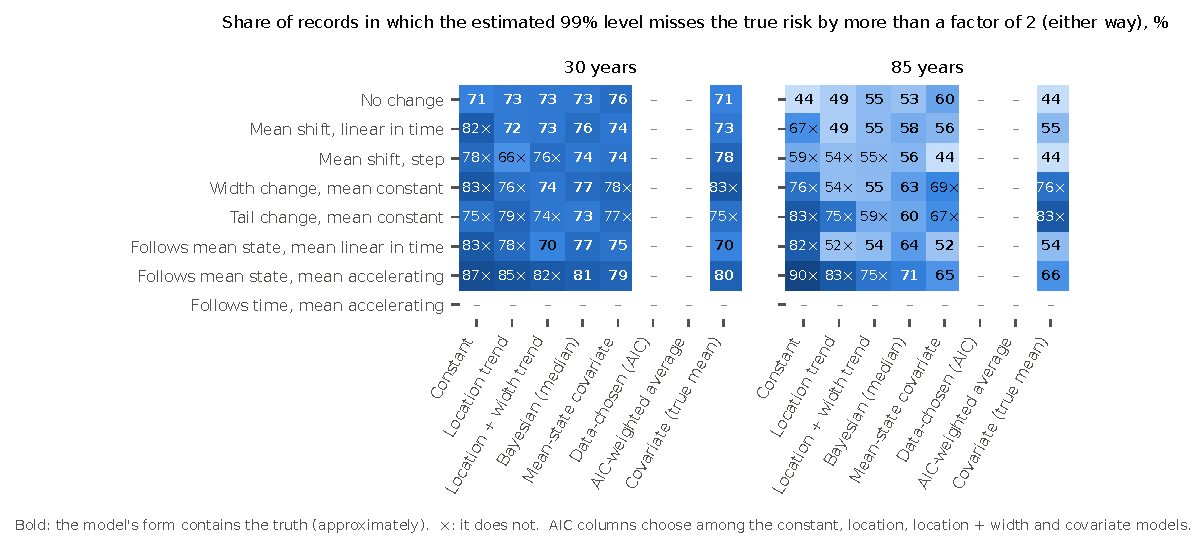
\includegraphics[width=\textwidth]{figures/fig_wrong_model.pdf}
\caption{Using the wrong model: share of records (\%) in which the estimated 1-in-100-year level of the last year misses the true risk by more than a factor of 2 either way (true probability of exceeding it above 2\% or below 0.5\%), by true process (rows) and fitted model (columns), at 30 and 85 years. Lighter is better. Bold: the model's form contains the true process (approximately); $\times$: it does not. AIC choice and AIC average: the model chosen by, or the Akaike-weighted average of, the constant, location-trend, location + width trend and mean-state covariate models. Oracle covariate: the covariate model given the true mean. At 85 years a model that cannot represent the true process usually misses more; at 30 years every model misses most records.}
\label{fig:wrong}
\end{figure}

\begin{table}[H]
\centering
\scriptsize
\setlength{\tabcolsep}{2.4pt}
\begin{tabular}{lrrrrrrrrrrr}
\toprule
 & \multicolumn{7}{c}{Missed by $>2\times$ either way, \% of records} & \multicolumn{4}{c}{AIC picks, \% of records} \\
\cmidrule(lr){2-8} \cmidrule(lr){9-12}
True process & Const. & Loc. & Loc.+wid. & Bayes & Cov. & AIC & AIC avg. & Const. & Loc. & Loc.+wid. & Cov. \\
\midrule
\multicolumn{12}{l}{\emph{30 yr}} \\
No change & \textbf{71} & \textbf{73} & \textbf{73} & \textbf{73} & \textbf{76} & -- & -- & 64 & 16 & 5 & 16 \\
Mean shift, linear in time & 82 & \textbf{72} & \textbf{73} & \textbf{76} & \textbf{74} & -- & -- & 40 & 44 & 8 & 9 \\
Mean shift, step & 78 & 66 & 76 & \textbf{74} & \textbf{74} & -- & -- & 27 & 53 & 5 & 15 \\
Width change, mean constant & 83 & 76 & \textbf{74} & \textbf{77} & 78 & -- & -- & 29 & 40 & 15 & 16 \\
Tail change, mean constant & 75 & 79 & 74 & \textbf{73} & 77 & -- & -- & 29 & 36 & 15 & 20 \\
Follows mean state, mean linear in time & 83 & 78 & \textbf{70} & \textbf{77} & \textbf{75} & -- & -- & 12 & 60 & 11 & 17 \\
Follows mean state, mean accelerating & 87 & 85 & 82 & \textbf{81} & \textbf{79} & -- & -- & 18 & 38 & 10 & 34 \\
Follows time, mean accelerating & -- & -- & -- & -- & -- & -- & -- & -- & -- & -- & -- \\
\multicolumn{12}{l}{\emph{85 yr}} \\
No change & \textbf{44} & \textbf{49} & \textbf{55} & \textbf{53} & \textbf{60} & -- & -- & 69 & 11 & 4 & 17 \\
Mean shift, linear in time & 67 & \textbf{49} & \textbf{55} & \textbf{58} & \textbf{56} & -- & -- & 22 & 59 & 2 & 17 \\
Mean shift, step & 59 & 54 & 55 & \textbf{56} & \textbf{44} & -- & -- & 6 & 20 & 2 & 72 \\
Width change, mean constant & 76 & 54 & \textbf{55} & \textbf{63} & 69 & -- & -- & 6 & 71 & 17 & 6 \\
Tail change, mean constant & 83 & 75 & 59 & \textbf{60} & 67 & -- & -- & 6 & 38 & 38 & 18 \\
Follows mean state, mean linear in time & 82 & 52 & \textbf{54} & \textbf{64} & \textbf{52} & -- & -- & 2 & 66 & 5 & 26 \\
Follows mean state, mean accelerating & 90 & 83 & 75 & \textbf{71} & \textbf{65} & -- & -- & 3 & 27 & 4 & 66 \\
Follows time, mean accelerating & -- & -- & -- & -- & -- & -- & -- & -- & -- & -- & -- \\
\bottomrule
\end{tabular}

\caption{Using the wrong model. Left: share of records (\%) in which the estimated 1-in-100-year level of the last year misses the true risk by more than a factor of 2 either way (true probability of exceeding it above 2\% or below 0.5\%); bold where the model's form contains the true process. Right: how often AIC selects each candidate. Const.: constant; Loc.: location trend; Loc.+wid.: location and width trend; Bayes: Bayesian posterior median; Cov.: mean-state covariate; AIC: the model chosen by AIC; AIC avg.: Akaike-weighted average. Appendix Table~\ref{tab:wrongdetail} splits the misses into under- and overstatement. The data rarely identify the true process, but the AIC-weighted average comes close to the best single model.}
\label{tab:wrong}
\end{table}

\paragraph{Findings.}
\begin{itemize}
\item \textbf{At 85 years the wrong driving variable makes the estimate clearly worse.} When the
  distribution follows an accelerating mean state, the location + width trend misses 75\% of
  records and the covariate model 65\%. When the width changes while the mean stays constant, the
  covariate model, whose covariate then carries no signal, misses 69\% and the location + width
  trend 55\%.
\item \textbf{Unneeded flexibility costs about as much.} With no change, the covariate model misses
  60\% of records against 44\% for the constant fit, because it fits a relation to the year-to-year
  noise of the annual mean; the location + width trend misses 55\%.
\item \textbf{Where the two kinds of model coincide, the choice hardly matters}: with the mean linear
  in time, with or without the distribution following it, the location trend, location + width
  trend and covariate model miss 49--56\% of records.
\item \textbf{A step favours the covariate model} (44\% against 54--55\% for the time trends),
  because the smoothed annual mean follows the step and a straight line cannot.
\item \textbf{For 30-year records the choice matters little}: every model misses 66--87\% of
  records, and within each true process the models differ by 5--13 points, while sampling noise
  alone causes 71\%.
\item \textbf{When the mean rises at an increasing rate, the mean-state model loses little even if the width follows
  time.} In the time-driven counterparts of the accelerating warming cases the covariate model's
  assumption about the width is wrong, yet it misses 64\% of 85-year records, against 68\% for the
  location + width trend and the Bayesian model and 71\% for the location trend. The time-trend
  models do better than when the width follows the mean (68\% against 75\% for the location + width
  trend), and the covariate model about the same (64\% against 65\%). Following the accelerating
  mean, which a straight line in time cannot, matters more than the driver of the width, which
  differs little between the two (Figure~\ref{fig:pworld}). The exception is the heavy-tailed $t$
  parent, whose change is mostly in the tail: there the location + width trend does better (48\%
  against 54\%). Our parametric time models are linear; a time model with a curved mean might do
  better, but we have not tested one.
\end{itemize}

\paragraph{Can the data tell?}
AIC selects among the constant, location-trend, location + width trend and covariate models
(Table~\ref{tab:wrong}, right). With 85 years it picks the covariate model in 66\% of the
accelerating mean-state cases and 72\% of the step cases, but also in 17\% of records with no change.
It almost never detects a width change: when only the width changes it picks the location trend in
71\% of records and the location + width trend in 17\%. When the width follows time rather than the
mean, it picks the covariate model less often (42\% against 66\%), so it leans the right way, but it
cannot reliably tell the two apart. With 30 years it picks the constant fit or the location trend in
most records whatever the truth.

Picking the lowest-AIC model is never far off, but it is sometimes 10 points worse than the best
single model: with no change it misses 54\% of 85-year records against 44\% for the constant fit,
and after a tail change 69\% against 59\%. Averaging the four models with Akaike weights does better
(Table~\ref{tab:wrong}). At 85 years it is within 4 points of the best single model for every true
process, and when the mean moves linearly it beats all of them (46\% against 49\% for the best). By
contrast, every single model, including the Bayesian one, is 11--30 points worse than the best for
at least one process. Over the standard cases it is also the best estimator at 85 years (51\%
missed against 56\% for the location trend, Section~\ref{sec:quant}), and in the covariate-model
cases it is close to the covariate model (64\% against 62\%, and 69\% for the location + width
trend). With 30 and 45 years the differences between all the choices are small,
and the average is within 6 points of the best model throughout.

\paragraph{What to do when we do not know.}
\begin{itemize}
\item \textbf{Do not expect the record to reveal the driver.} The time and mean-state models
  coincide whenever the mean moves linearly in time, and AIC rarely detects a width change. Whether
  the change follows time or the mean state has to come from physical reasoning or from evidence
  outside the record.
\item \textbf{Average rather than choose.} An AIC-weighted average of the constant, time-trend and
  mean-state models gives up a few points against the best model for the true process, whatever that
  is, and avoids the large losses of committing to a wrong one.
\item \textbf{When the mean clearly moves nonlinearly, include a mean-state model.} With an
  accelerating mean or a step, the covariate model did best whether or not the width followed the
  mean.
\item \textbf{Report the spread between plausible models} as part of the uncertainty of the current
  return level, alongside the sampling uncertainty of each.
\item \textbf{With 30 years, the model matters less than the data.} Two-thirds or more of 30-year
  records miss the current 99\% level by a factor of 2 whatever is fitted; only longer records or
  additional information (other sites, or more declustered values per year) are likely to change
  that.
\end{itemize}

\begin{figure}[H]
\centering
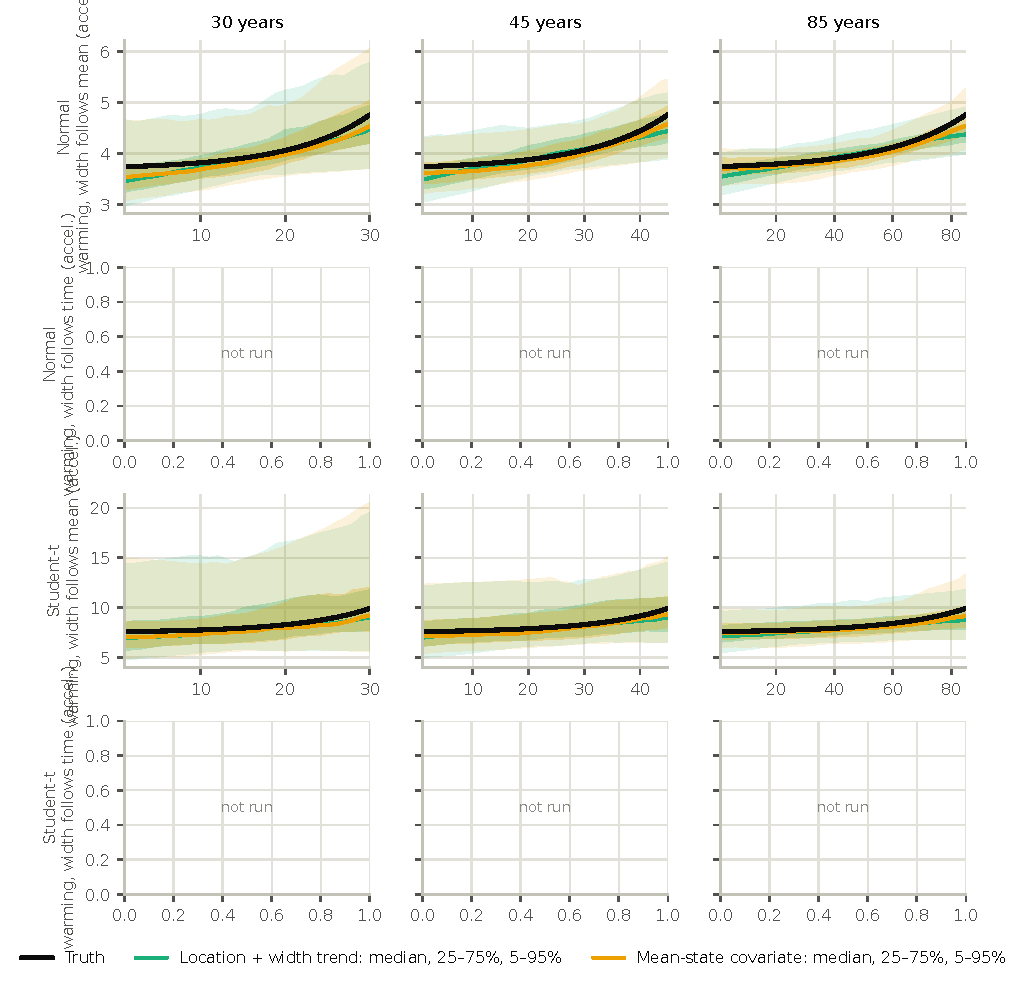
\includegraphics[width=\textwidth]{figures/fig_paths_world.pdf}
\caption{The same accelerating warming reached in two ways: the width (and for the Student-$t$ the tail) follows the mean state (``width follows mean''), or changes linearly in time between the same first- and last-year distributions (``width follows time''). Rows: normal and Student-$t$ parents in each world; columns: record length. Green: location + width trend; yellow: mean-state covariate model (same number of parameters). In each year: median of the 100 estimates (line), 25--75\% (dark band) and 5--95\% (light band); black: the truth. Units: baseline daily standard deviation. The two models differ little compared with the spread across records.}
\label{fig:pworld}
\end{figure}

\begin{figure}[H]
\centering
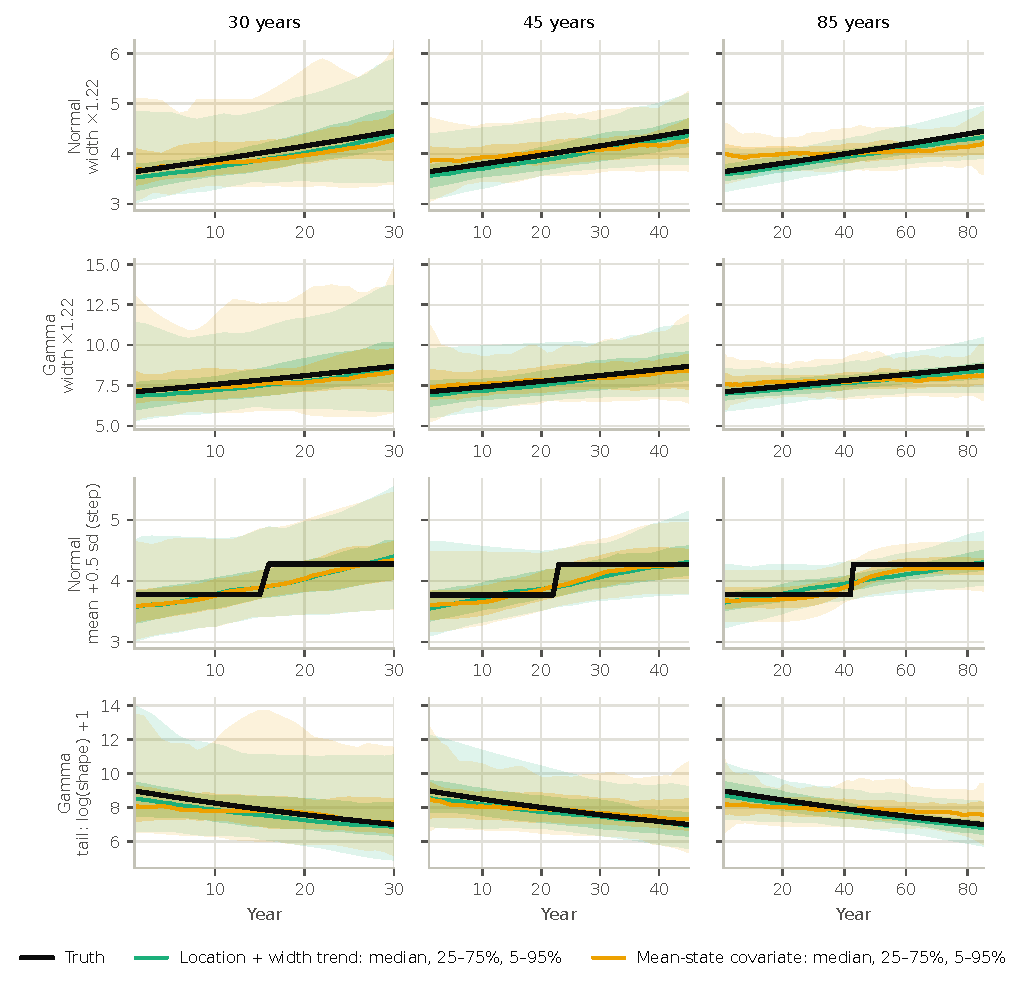
\includegraphics[width=\textwidth]{figures/fig_paths_wrong.pdf}
\caption{Cases in which the mean state does not track the change: width or tail changes at constant mean, and a step in the mean. Green: location + width trend; yellow: mean-state covariate model. In each year: median of the 100 estimates (line), 25--75\% (dark band) and 5--95\% (light band); black: the truth. Columns: record length. Units: baseline daily standard deviation. With a width or tail change the covariate model sees little signal and its path is flatter than the truth; for the step it follows the smoothed step.}
\label{fig:pwrong}
\end{figure}

\paragraph{Single records.}
Figure~\ref{fig:rwrong} shows typical single records for six of the processes, with the location +
width trend, the covariate model and the AIC-weighted average. When the width changes at constant
mean, the covariate model stays almost flat and understates the current risk (4.9\%), while the
location + width trend follows the widening (1.8\%). After a step the covariate model follows the
smoothed step. With accelerating warming the covariate model ends closer to the truth than the
location + width trend whether the width follows the mean (2.7\% against 5.4\%) or time (2.5\%
against 3.3\%). The AIC-weighted average usually lies between the two.

\begin{figure}[H]
\centering
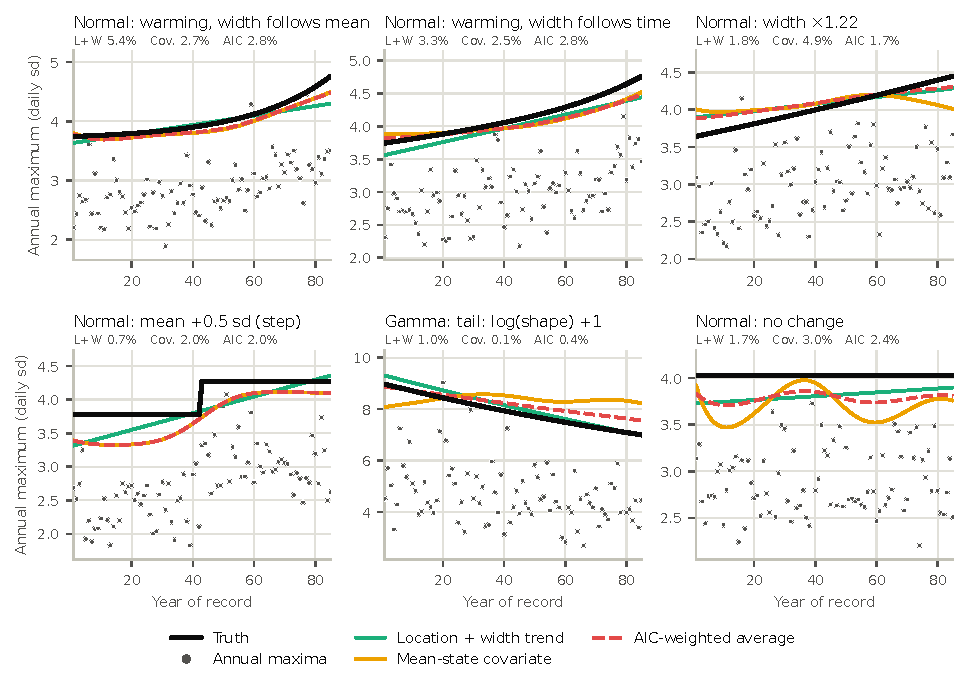
\includegraphics[width=\textwidth]{figures/fig_records_wrong.pdf}
\caption{Typical 85-year records for six true processes (panel titles). ``Typical'': the median of 100 records ranked by the average error of the three estimates shown in the last year, $|\log(\text{true exceedance}/1\%)|$. Points: annual maxima; black: true 1-in-100-year level; green: location + width trend; yellow: mean-state covariate model; red, dashed: AIC-weighted average. Above each panel: the true probability that each estimate of the last year's level is exceeded (ideal 1\%; above 2\%: risk understated at least twofold; below 0.5\%: overstated; L+W: location + width trend, Cov.: covariate model, AIC: AIC-weighted average). Units: baseline daily standard deviation.}
\label{fig:rwrong}
\end{figure}

\paragraph{The covariate-model cases in detail.}
In these cases the width and tail of the daily distribution change with the mean, and the mean
itself rises along an accelerating path. At 85 years the location trend misses the current risk by
more than a factor of 2 in 74\% of records, almost all by understating it (71\%); the location +
width trend and the Bayesian model miss 69\% (60\% and 57\% understated). The covariate model does
clearly better (62\%: 45\% understated, 16\% overstated), as well as its oracle version with the true
mean path (63\%). Two things contribute: the covariate
captures the acceleration, which a straight line in time cannot, and it is estimated from all daily
values, not only the extremes, so it is much less noisy than the extremes themselves. Letting the
tail index also depend on the covariate makes things worse (80\%), because the tail index then
follows the noise in the covariate.

Figures~\ref{fig:pwarm} and \ref{fig:pwet} show the paths. The covariate model (yellow) follows
the accelerating rise; the location trend (blue), a straight line, cuts across it and ends well below
the truth (by 0.4 daily sd for the normal parent, 40\% of the true change), and this shortfall
does not shrink with record length, because it comes from the form of the model, not from noise.
The covariate model's median also ends somewhat low (by 0.2), but so does its oracle version with the
true mean as covariate (by 0.14): this is mostly the downward tendency of a typical high-quantile
estimate seen already in the no-change case. Its bands widen at the end of short records, where the
smoothed covariate is least certain. For the $t$ parent, whose tail gets heavier as it warms, the
shortfall is larger (0.8 against 1.5 for the location trend), because the model holds the tail index
constant.

\begin{figure}[H]
\centering
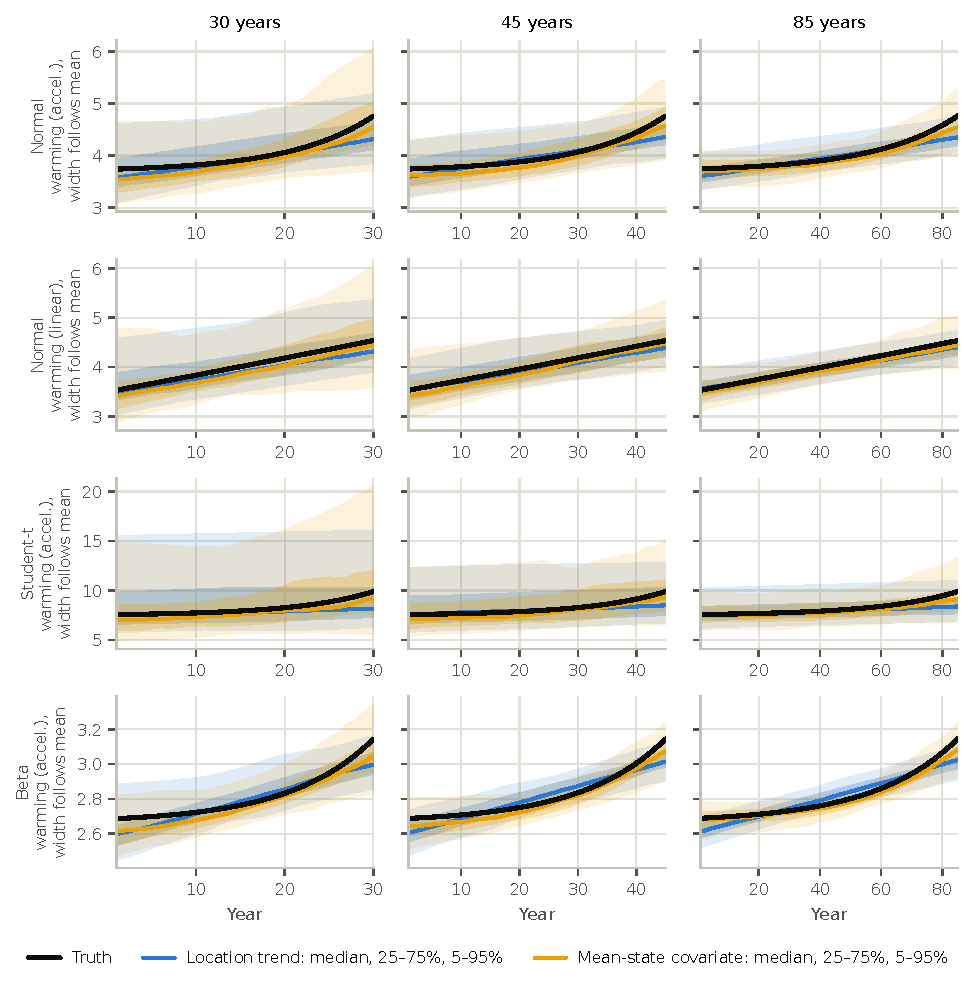
\includegraphics[width=\textwidth]{figures/fig_paths_warming.pdf}
\caption{Temperature-like covariate-model cases: the mean rises (at an accelerating rate, or linearly in the second row), and the width (and for the Student-$t$ and beta the tail) follows it. Rows: parent; columns: record length (same total change in each). Blue: location trend; yellow: mean-state covariate model. In each year: median of the 100 estimates (line), 25--75\% (dark band) and 5--95\% (light band); black: the truth. Units: baseline daily standard deviation. Where the mean accelerates, the covariate model follows it and the linear trend lags at the end of the record.}
\label{fig:pwarm}
\end{figure}
\begin{figure}[H]
\centering
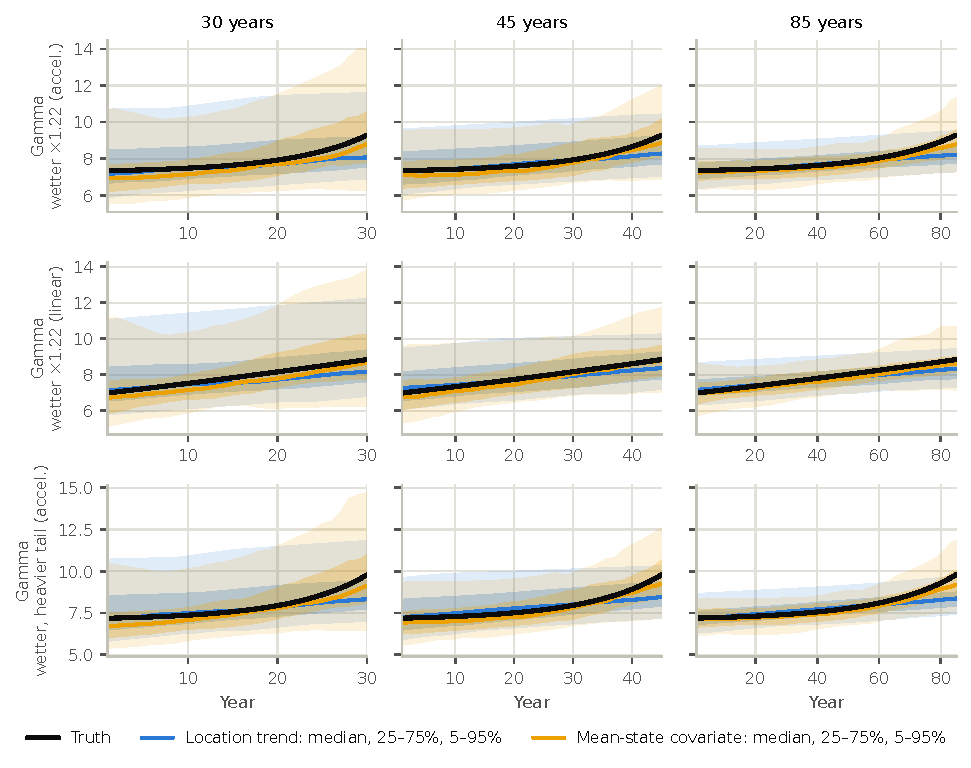
\includegraphics[width=\textwidth]{figures/fig_paths_wetter.pdf}
\caption{Precipitation-like covariate-model cases (gamma parent): every quantile scales with an accelerating mean, and in the last row the tail also gets heavier. Columns: record length (same total change in each). Blue: location trend; yellow: mean-state covariate model. In each year: median of the 100 estimates (line), 25--75\% (dark band) and 5--95\% (light band); black: the truth. Units: baseline daily standard deviation.}
\label{fig:pwet}
\end{figure}


%=====================================================================================
\section{The Bayesian random-walk model}\label{sec:bayes}

\paragraph{Credible intervals.}
The 90\% intervals for the last year's $\Xp$ contain the truth in 94--100\% of records, so they
are conservative (Figure~\ref{fig:bayes}). Their median width is 1.3 to 3 times the 5--95\% range
of the actual errors of the posterior median. The intervals are honest but too wide to be
informative for short records.

\begin{figure}[H]
\centering
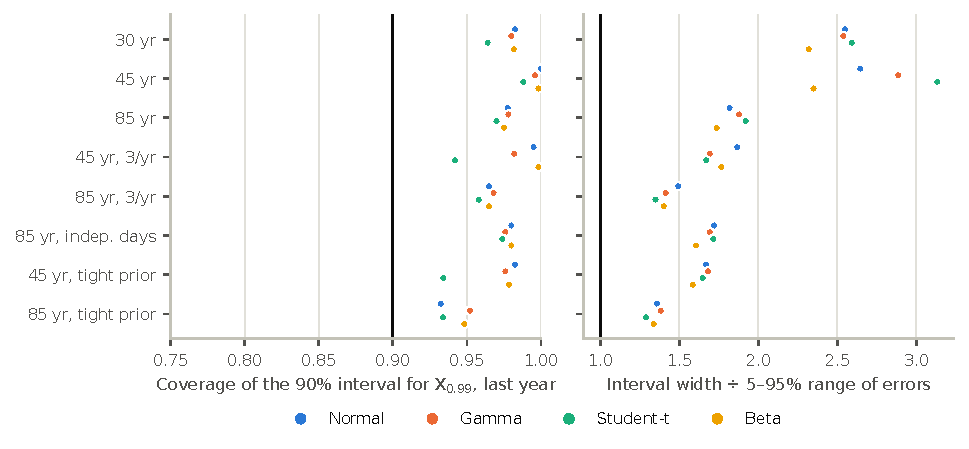
\includegraphics[width=\textwidth]{figures/fig09_bayes_intervals.pdf}
\caption{Bayesian random-walk model, standard cases, by design (rows; 3/yr: three values per year; indep.\ days: no day-to-day correlation; tight prior: random-walk prior scales 0.25). Left: coverage, the share of records whose 90\% credible interval for the last year's 1-in-100-year level contains the truth (nominal 0.90, vertical line). Right: median interval width divided by the 5--95\% range of the actual errors of the posterior median (1 = right width). One dot per parent distribution. The intervals cover the truth more often than nominal because they are 1.3 to 3 times too wide.}
\label{fig:bayes}
\end{figure}

\paragraph{Convergence.}
Under the authors' prior most fits have some divergent transitions (median 9 of 4,000 at
85 years and 81 at 30 years). With one value per year, R-hat exceeds 1.05 in fewer than 1\% of
fits. With three values per year it exceeds 1.05 in 10--12\% of fits, almost always far above
(R-hat $>1.5$, chains in different modes), and these are concentrated in the bounded beta parent
(25--32\% of its fits). Our chains are shorter than the authors', but disagreement between chains
of this size is not a matter of chain length. The unconverged fits overstate the risk more often than the converged ones (37--49\% against
19--32\% overstated twofold), but they are a minority, and excluding them changes the pooled shares
by at most 2 points.

\paragraph{Prior sensitivity.}
Shrinking the random-walk scales for $\xi$, $\alpha$ and $s$ to 0.25 nearly eliminates the
convergence problems (R-hat $\le1.05$ in every fit, median 1--6 divergences). It improves accuracy
slightly at 85 years (56\% of records missed against 59\%, mostly because fewer are understated:
35\% against 39\%), leaves 45 years unchanged (70\%), and brings interval coverage closer to nominal (93--98\%). See Appendix Figure~\ref{fig:prior}.
Figure~\ref{fig:pprior} shows the cost: the tighter prior narrows the bands, but it also makes the
paths stiffer, so for the $t$ tail change the median follows less of the early, high values.
Figure~\ref{fig:ppriorcov} compares both priors with the covariate model in the covariate-model
cases. There the tighter prior misses as many records as the authors' (69\% at 85 years, against
62\% for the covariate model), more of them by understating the risk (60\% against 57\%), and its
intervals cover the truth in only 88\% of records (80--92\% by
case), because its stiffer paths lag the acceleration at the end of the record.

\begin{figure}[H]
\centering
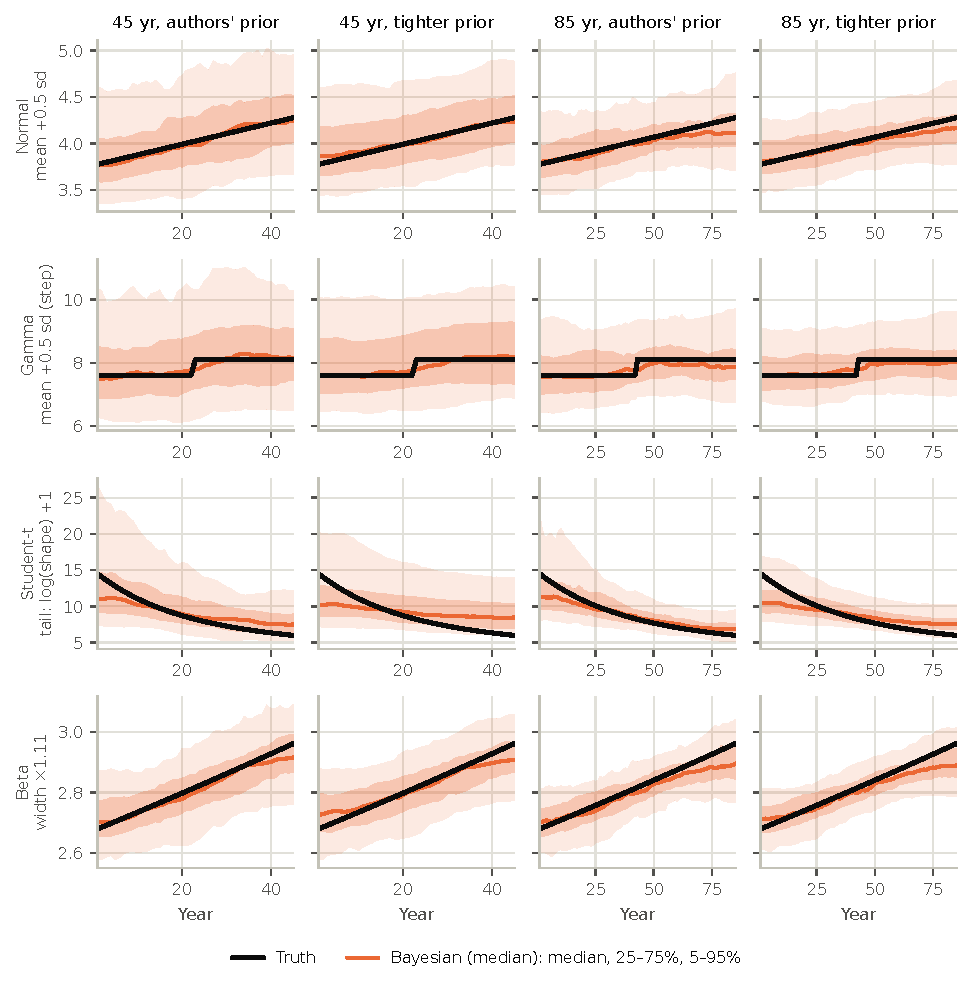
\includegraphics[width=\textwidth]{figures/fig_paths_prior.pdf}
\caption{Bayesian posterior median with the authors' prior and with a tighter prior on the random-walk scales (0.25 instead of 1, 0.5, 0.5), at 45 and 85 years (columns), for four cases (rows). In each year: median of the 100 posterior medians (line), 25--75\% (dark band) and 5--95\% (light band); black: the truth. Units: baseline daily standard deviation. The tighter prior narrows the bands but makes the paths stiffer, so they follow less of a change.}
\label{fig:pprior}
\end{figure}
\begin{figure}[H]
\centering
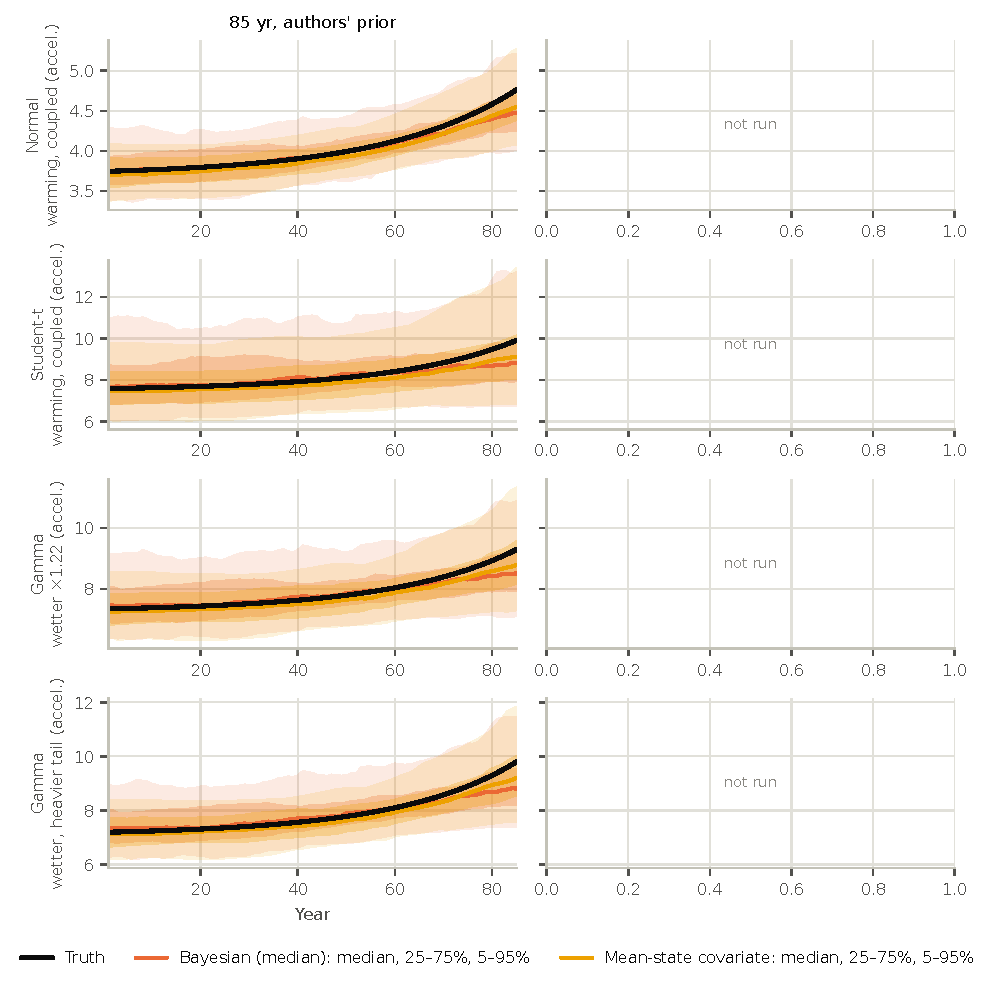
\includegraphics[width=\textwidth]{figures/fig_paths_prior_covariate.pdf}
\caption{Covariate-model cases at 85 years (rows; width and tail follow an accelerating mean): Bayesian posterior median (orange) with the authors' and the tighter prior (columns), and the mean-state covariate model (yellow). In each year: median of the 100 estimates (line), 25--75\% (dark band) and 5--95\% (light band); black: the truth. Units: baseline daily standard deviation. The tighter prior's stiffer paths lag the acceleration at the end of the record.}
\label{fig:ppriorcov}
\end{figure}


\paragraph{Time reversal.}
The model's prior is symmetric in time, so fitting a record in reverse order should give the
reversed posterior paths. For four test cases the largest difference between the forward and
reversed posterior medians of $\Xp$ was 0.003--0.11, at most 1\% of the width of the 90\%
interval, consistent with MCMC noise.

%=====================================================================================
\section{The posterior-predictive 1-in-100-year level}\label{sec:pred}

A Bayesian posterior offers a second way to state the current 1-in-100-year level. Instead of a
statistic (median or mean) of the levels implied by the individual posterior draws, one can
average the draws' distributions into a single posterior predictive distribution and take its
99th percentile. We call this \emph{the predictive level}. It is a single, well-defined number, it
is what a learner who holds the posterior should use to price a contract that pays when the level
is exceeded, and it is the natural choice in risk applications. This section asks how
close it is to the truth and where its uncertainty comes from. We refitted every Bayesian run of
Section~\ref{sec:quant} with its original seeds and settings (19,700 fits), keeping the
draws' distributions; the posterior medians and means reproduce the earlier fits to within
$3\times10^{-6}$, so all comparisons below are on the same records and draws.

The predictive level answers a different question from the estimators of
Section~\ref{sec:quant}. They try to estimate a fixed but unknown number, the true $\Xp$, and
the posterior median is the Bayesian model's best estimate of it. The predictive level instead
states a risk: under everything the posterior still believes, including draws with heavy tails,
the chance of exceeding it is 1\%. Because it folds parameter uncertainty into the level, it lies
above the posterior median by design, and lying above the true level is not in itself a fault. We score it the same way as the estimators, by the true chance of exceeding it, because that
is what a user relying on it is exposed to. The question is whether the margin it builds in is the
right size, and how much it varies from one record to the next.

\subsection{Definition}\label{sec:pred-what}


The model gives, for each posterior draw $d=1,\dots,D$, GEV parameters
$\theta_d(t)=(\mu_d(t),\sigma_d(t),\xi_d(t))$ for the annual maximum in year $t$. The draw's own
99th percentile is $q_d(t)$, with $P(Y_t>q_d(t)\mid\theta_d)=1\%$. The \emph{posterior median}
estimate is the median of the $q_d(t)$ over draws. The \emph{predictive level} $\xs(t)$ instead
solves
\begin{equation}
\frac1D\sum_{d=1}^{D} P\bigl(Y_t>\xs(t)\mid\theta_d(t)\bigr)=1\%,
\end{equation}
the 99th percentile of the posterior predictive distribution of the year-$t$ maximum. It averages
probabilities, not levels. Since a probability cannot go above 1 but can fall to zero, and the
upper tail of a GEV distribution is very sensitive to $\xi$, the average is pulled up by the draws
with the heaviest tails: in our records $\xs$ is above the posterior median in every record, and
above the posterior mean of $q_d$ in two-thirds of records at 85 years (a tenth at 30 years;
Figure~\ref{fig:pred-anatomy}).

Throughout, the quantity studied is this predictive 99th percentile of the annual-maximum
distribution, i.e.\ the 1-in-100-year level, in the final year of the record. A predictive
percentile of another quantity (daily rainfall, say) works by the same mechanism, but its numbers
will differ.

\subsection{How close is the predictive level to the truth?}\label{sec:pred-close}

Table~\ref{tab:pred-designs} and Figure~\ref{fig:pred-exceedance} give the main result, pooled over the
standard cases (the four distributions with and without change).

\begin{table}[H]
\centering\small\setlength{\tabcolsep}{3.5pt}
\caption{Predictive level: the 99th percentile of the Bayesian model's posterior predictive distribution of the last year's annual maximum (Section~\ref{sec:pred}). Standard cases, 2,000 records per design (3/yr: three values per year; indep.\ days: no day-to-day correlation; tight prior: random-walk prior scales 0.25). Left, for the predictive level: median and average over records of its true exceedance probability (the true chance that the last year's annual maximum exceeds it; ideal 1\%); under: share of records (\%) with the risk understated at least twofold (true exceedance above 2\%, level too low); over: overstated at least twofold (below 0.5\%, level too high); missed = under + over. Middle: share missed by other estimators on the same records. Right: missed share of the predictive level minus that of the posterior median, in percentage points $\pm$ one standard error. The predictive level is about right on average but usually too high in a single record.}\label{tab:pred-designs}
\begin{tabular}{l rrrrr rrr r}
\toprule
 & \multicolumn{5}{c}{Bayes, predictive} & \multicolumn{3}{c}{Missed, others} & \\
\cmidrule(lr){2-6}\cmidrule(lr){7-9}
Design & median & avg. & under & over & \textbf{missed} & \shortstack{post.\\median} & \shortstack{loc.\\trend} & \shortstack{AIC\\avg.} & \shortstack{pred.\ $-$\\median} \\
\midrule
30 yr & 0.01\% & 0.5\% & 8 & 84 & \textbf{92} & 75 & 73 & 75 & $+17\pm1$ \\
45 yr & 0.05\% & 0.4\% & 6 & 78 & \textbf{84} & 70 & 69 & 69 & $+14\pm1$ \\
85 yr & 0.4\% & 0.8\% & 12 & 56 & \textbf{68} & 59 & 56 & 51 & $+9\pm2$ \\
85 yr, 3/yr & 0.5\% & 0.9\% & 13 & 53 & \textbf{66} & 55 & 55 & 46 & $+11\pm2$ \\
85 yr, indep. days & 0.3\% & 0.8\% & 13 & 58 & \textbf{71} & 65 & 58 & 55 & $+6\pm2$ \\
45 yr, tight prior & 0.2\% & 0.7\% & 11 & 63 & \textbf{74} & 70 & 69 & 69 & $+4\pm1$ \\
85 yr, tight prior & 0.6\% & 1.1\% & 16 & 42 & \textbf{57} & 56 & 56 & 51 & $+1\pm1$ \\
\bottomrule
\end{tabular}

\end{table}

\begin{figure}[H]
\centering
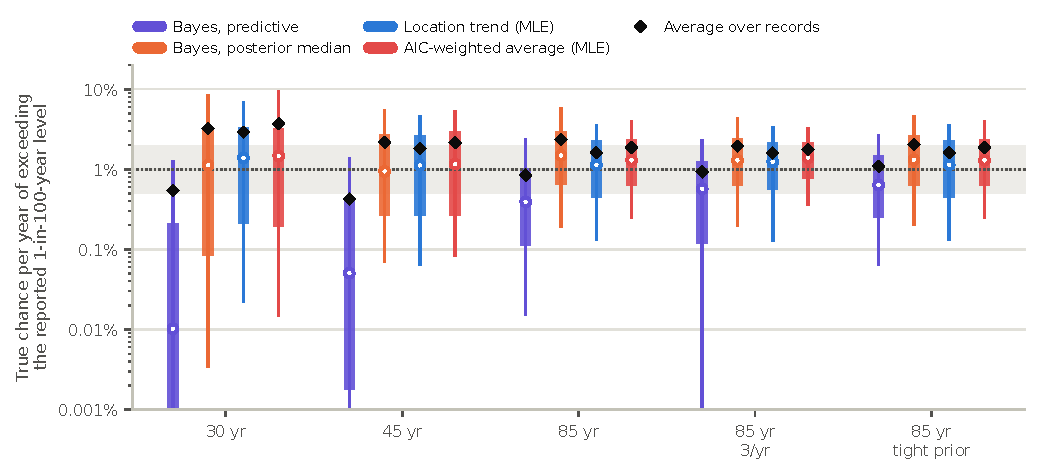
\includegraphics[width=\textwidth]{figures/pred_exceedance.pdf}
\caption{True probability that the last year's annual maximum exceeds the reported 1-in-100-year level (ideal 1\%, dotted line), over the records of the standard cases. Violet: the Bayesian posterior-predictive level; orange: Bayesian posterior median; blue: location-trend fit; red: AIC-weighted average. White circle: median over records; black diamond: average; thick bar: 25--75\%; thin bar: 10--90\%. Grey band: within a factor of 2 of 1\% (0.5--2\%); below it the level is too high (risk overstated), above it too low (understated). Groups: record length, three values per year (3/yr) and the tighter prior. The predictive level is near 1\% on average, but its median is far lower: in a typical record it overstates the risk.}\label{fig:pred-exceedance}
\end{figure}

\begin{itemize}
\item \textbf{The predictive level is usually too high.} Its median true exceedance is 0.39\% at 85
  years, 0.05\% at 45 and 0.01\% at 30. The other estimators are centred near 1\% (medians 0.9--1.5\%).
\item \textbf{It misses more often.} It is off by more than a factor of 2 in 68\% of records at
  85 years, 84\% at 45 and 92\% at 30, almost always by overstating. The posterior median misses in
  59\%, 70\% and 75\%, the location trend in 56\%, 69\% and 73\%.
\item \textbf{The dispersion is larger, and lopsided.} At 85 years the middle 80\% of its true
  exceedances runs from 0.015\% to 2.4\%, a factor of about 160; for the posterior median it is 0.19\%
  to 6\%, a factor of about 30. At 30 years, a tenth of predictive levels have essentially no chance of
  being exceeded in the simulated climate.
\item \textbf{The level itself is not far off; the probability is.} In the precipitation-like
  (gamma) records, the predictive 100-year depth is a median 8\% above the true depth at 85 years
  (10--90th percentile $-6\%$ to $+25\%$), 22\% above at 45 years and 31\% above at 30. Because the
  chance of exceedance falls steeply with depth in the far tail, an 8\% overstatement of the depth
  becomes a factor of 2.5 in the probability.
\item \textbf{Several values per year help, but only modestly.} Fitting the three largest
  (declustered) values of each year instead of the annual maximum cuts the share of records whose
  posterior leans heavy-tailed from 38\% to 14\% at 45 years and from 12\% to 8\% at 85 years
  (Table~\ref{tab:pred-uncertainty}). The predictive level's median true exceedance rises from 0.05\% to
  0.2\% at 45 years and from 0.4\% to 0.6\% at 85, and its share missed falls from 84\% to 78\% and
  from 68\% to 60\%. But the other estimators gain about as much, so the predictive level still
  misses 7--16 points more often than the posterior median.
\end{itemize}

Table~\ref{tab:pred-groups} breaks the 85-year results down by the kind of change and by distribution.
The predictive level overstates the risk more often than it understates it in every kind of case, including no
change at all. It does about as well as the posterior median only where the true change widens the
distribution or makes its upper tail heavier, so that the other estimators tend to understate the
risk: in the width cases (64\% missed, against 63\%) and when the spread and tail follow a rising
mean (68\% against 69\%). It does worst where the tail becomes lighter (79\% missed).

\begin{table}[H]
\centering\small\setlength{\tabcolsep}{3.5pt}
\caption{The posterior-predictive level at 85 years by kind of change (top) and by parent distribution (bottom, standard cases only). Records: number of records. Median: median true exceedance probability of the predictive level (ideal 1\%). Under and over: share of records (\%) in which the risk is understated (true exceedance above 2\%, level too low) or overstated (below 0.5\%, level too high) at least twofold; missed = under + over. Right: share missed by other estimators on the same records. Follows mean state: width and tail follow an accelerating mean; time-driven: the same end states reached linearly in time. The predictive level overstates more often than it understates in every kind of case.}\label{tab:pred-groups}
\begin{tabular}{l r rrr r rrr}
\toprule
 & & \multicolumn{4}{c}{Bayes, predictive} & \multicolumn{3}{c}{Missed, others} \\
\cmidrule(lr){3-6}\cmidrule(lr){7-9}
Kind of change & records & median & under & over & \textbf{missed} & \shortstack{post.\\median} & \shortstack{loc.\\trend} & \shortstack{AIC\\avg.} \\
\midrule
No change & 400 & 0.5\% & 11 & 52 & \textbf{64} & 53 & 49 & 47 \\
Mean & 800 & 0.4\% & 14 & 54 & \textbf{67} & 57 & 52 & 45 \\
Width & 400 & 0.6\% & 19 & 46 & \textbf{64} & 63 & 54 & 54 \\
Tail & 300 & 0.2\% & 3 & 76 & \textbf{79} & 60 & 75 & 62 \\
Position (beta) & 100 & 0.2\% & 11 & 66 & \textbf{77} & 76 & 73 & 61 \\
Follows mean state & 700 & 0.6\% & 24 & 45 & \textbf{68} & 69 & 74 & 64 \\
Time-driven & 300 & 0.6\% & 24 & 47 & \textbf{71} & 68 & 71 & 65 \\
\midrule
Normal (standard cases) & 400 & 0.5\% & 15 & 50 & \textbf{65} & 60 & 50 & 46 \\
Gamma (standard cases) & 500 & 0.4\% & 11 & 56 & \textbf{67} & 53 & 50 & 47 \\
Student-t (standard cases) & 500 & 0.4\% & 9 & 55 & \textbf{64} & 50 & 56 & 46 \\
Beta (standard cases) & 600 & 0.3\% & 15 & 60 & \textbf{75} & 70 & 66 & 60 \\
\bottomrule
\end{tabular}

\end{table}

\subsection{The average versus a single record}\label{sec:pred-average}

The predictive level does what it is built to do on average: the true chance of exceeding it,
averaged over records, is 0.85\% at 85 years (0.43--0.55\% at 30--45 years), the closest to 1\% of
the estimators we tested, alongside the posterior mean; the posterior median and the
maximum-likelihood fits average 1.6--3.7\% (diamonds in Figure~\ref{fig:pred-exceedance}).
But the average is carried by a minority of records in which the level is too low, while in the
typical record it is far too high.

This is the familiar gap between the average and the typical value of a skewed quantity. For a
risk taker who writes many independent contracts and cares only about the expected total, the
average is the relevant number, and by that standard the predictive level is well calibrated or
conservative. For a single contract, location or portfolio exposed to one climate, the typical
record is more relevant, and there the predictive level usually implies a risk several times
higher than the true one. Climate risks at nearby locations are strongly correlated, and a model and
prior applied in the same way everywhere will err in the same direction everywhere, so the
diversification that would make the average relevant is limited.

A Bayesian predictive distribution is calibrated in this average sense when the true climates are
drawn from the prior. Our synthetic climates are not drawn from the authors' prior: the GEV shape
of their annual maxima is at most about 0.2 (the Student-$t$ case), whereas the prior allows $\xi$
up to 2.1, and above $\xi=1$ even the mean of the distribution is infinite. To the extent that real
rainfall extremes have lighter tails than the prior allows, the same overstatement should be
expected in real records.

\subsection{Pricing cover with a known 1\% risk}\label{sec:pred-price}

Figure~\ref{fig:pred-price} turns the question around: for the level whose true chance of being
exceeded is exactly 1\% in the final year, what chance does each model assign? That chance is the
pure premium rate the model would charge for cover triggered at that level.

\begin{figure}[H]
\centering
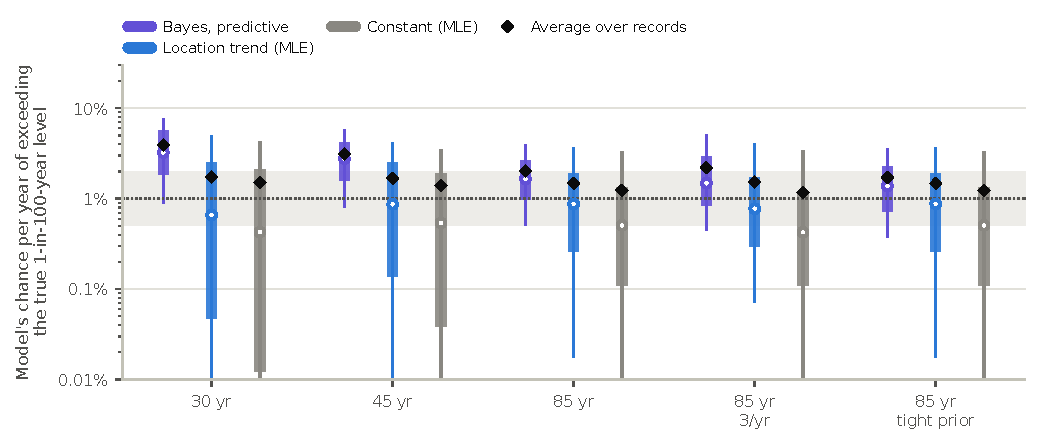
\includegraphics[width=\textwidth]{figures/pred_price.pdf}
\caption{Pricing cover for an event whose true chance is 1\% a year: each model's probability (its pure premium rate) that the last year's annual maximum exceeds the true 1-in-100-year level, over the records of the standard cases. Violet: Bayesian posterior predictive; blue: location trend; grey: constant GEV. White circle: median over records; diamond: average; thick bar: 25--75\%; thin bar: 10--90\%. Grey band: within a factor of 2 of the true 1\%; above it the model overprices, below it underprices. The predictive model rarely underprices but usually overprices; the trend fit is right on average but often underprices tenfold or more.}\label{fig:pred-price}
\end{figure}

\begin{itemize}
\item \textbf{The predictive model charges too much, but rarely too little.} Its median rate is 1.7\%
  at 85 years, 2.8\% at 45 and 3.2\% at 30. It charges less than 0.5\% in only 4--10\% of records
  and less than 0.1\% almost never; it charges more than 2\% in 40\% of records at 85 years and in
  67--72\% at 30--45 years.
\item \textbf{A trend fit is right on average but often dangerously low.} The location-trend
  maximum-likelihood fit has a median rate of 0.7--0.9\%, but charges less than 0.5\% in 36--45\% of
  records and less than 0.1\% in 16--28\%: in those records the cover would be priced at a tenth or
  less of its true cost.
\item The predictive approach therefore trades frequent and large over-pricing for protection
  against severe under-pricing. Whether that is a good trade is a question about risk preferences;
  the point here is that the loading it implies is large, varies by a factor of several from one
  record to the next, and is set mainly by the prior (Section~\ref{sec:pred-prior}).
\end{itemize}

\subsection{Where the uncertainty comes from}\label{sec:pred-sources}

\paragraph{The posterior's own spread.}

Figure~\ref{fig:pred-anatomy} shows one typical precipitation-like record of 85 years with no change.
Left: each grey curve is the chance of exceeding a given level under one posterior draw. The draws
fan out in the tail. The predictive curve (violet) is their average; it lies above most of the
draws because the few heavy-tailed ones dominate the average in the far tail. Right: the
distribution over draws of the chance of exceeding the predictive level. By construction it
averages 1\%, but the median draw gives 0.40\%, close to the truth (0.48\%), and the top 5\% of
draws carry a third of the average.

\begin{figure}[H]
\centering
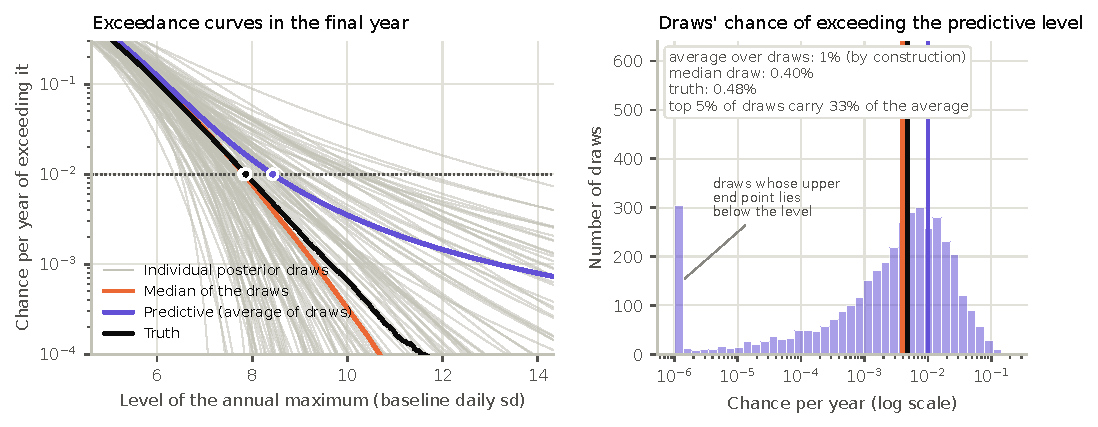
\includegraphics[width=\textwidth]{figures/pred_anatomy.pdf}
\caption{Why the posterior-predictive level lies high, in one record (gamma, precipitation-like parent, 85 years, no change; the record whose predictive level has the median true exceedance of its case). Left: chance per year that the annual maximum exceeds a given level, under each of 120 posterior draws (grey), their median (orange), their average, which is the posterior predictive curve (violet), and the truth (black); dots mark where each curve crosses 1\%. The few heavy-tailed draws dominate the average far in the tail, so the predictive curve crosses 1\% at a higher level. Right: histogram over all draws of each draw's chance of exceeding the predictive level (log scale; draws at or below $10^{-6}$ are gathered in the leftmost bar). By construction they average 1\%, but the median draw gives 0.40\%, close to the truth (0.48\%).}\label{fig:pred-anatomy}
\end{figure}

Table~\ref{tab:pred-uncertainty} summarises this over all records. The posterior is honest about its
uncertainty: the true chance lies within the draws' 5--95\% range in 96--100\% of records. But the
range is very wide, from essentially 0 to about 5\%, so the single number hides a very wide spread
of beliefs. ``Dominated by a few draws'' is accurate in a specific sense: the top 5\% of draws
carry 38\% (85 years) to 52\% (30 years) of the 1\%, and the effective number of draws that
determine the average is 13--21\% of the total.

\begin{table}[H]
\centering\small\setlength{\tabcolsep}{3pt}
\caption{How uncertain the posterior is about the risk at its own predictive level, standard cases, by design. Each posterior draw implies a chance of exceeding the predictive level; by construction these average 1\%. Draws' chance: the 5th, 50th and 95th percentiles of these over the draws (median over records). Heavy-tailed: share of records in which more than 5\% of the draws have GEV shape $\xi>0.5$ (the true $\xi$ is at most about 0.2 in our climates). Truth inside: share of records in which the true exceedance probability lies inside the draws' 25--75\% (50\%) and 5--95\% (90\%) ranges. Top 5\%: share of the 1\% average contributed by the 5\% of draws with the highest values (median over records). Monte Carlo: typical multiplicative error of the predictive level's exceedance probability with 4,000 draws, from the spread between the four chains. A typical draw puts the risk well below 1\%; a few put it at several percent.}\label{tab:pred-uncertainty}
\begin{tabular}{l rrr r rr r r}
\toprule
 & \multicolumn{3}{c}{\shortstack{Draws' chance of\\exceeding the level}} & & \multicolumn{2}{c}{\shortstack{Truth\\inside}} & & \\
\cmidrule(lr){2-4}\cmidrule(lr){6-7}
Design & 5\% & median & 95\% & \shortstack{heavy-\\tailed} & 50\% & 90\% & \shortstack{top\\5\%} & \shortstack{Monte\\Carlo} \\
\midrule
30 yr & 0.00\% & 0.00\% & 5.8\% & 53\% & 64\% & 96\% & 52\% & $\times$1.11 \\
45 yr & 0.00\% & 0.04\% & 5.4\% & 38\% & 69\% & 100\% & 47\% & $\times$1.10 \\
85 yr & 0.00\% & 0.2\% & 4.6\% & 12\% & 67\% & 98\% & 38\% & $\times$1.06 \\
45 yr, 3/yr & 0.00\% & 0.2\% & 4.5\% & 14\% & 69\% & 98\% & 35\% & $\times$1.06 \\
85 yr, 3/yr & 0.00\% & 0.4\% & 3.9\% & 8\% & 65\% & 97\% & 27\% & $\times$1.04 \\
85 yr, indep. days & 0.00\% & 0.2\% & 4.6\% & 17\% & 61\% & 98\% & 38\% & $\times$1.06 \\
45 yr, tight prior & 0.00\% & 0.3\% & 4.4\% & 18\% & 54\% & 97\% & 34\% & $\times$1.06 \\
85 yr, tight prior & 0.00\% & 0.5\% & 3.8\% & 4\% & 57\% & 96\% & 28\% & $\times$1.03 \\
\bottomrule
\end{tabular}

\end{table}

\paragraph{The tail shape.}

Which records are overstated most? Those whose posterior leans towards heavy tails
(Figure~\ref{fig:pred-xi}). The true GEV shape of the annual maxima in our climates ranges from about
$-0.25$ (bounded) to about $+0.17$ (Student-$t$); with 30--45 years of data the posterior mean of $\xi$
is often well above that, and every positive shift in $\xi$ raises the predictive level steeply.
At 30 years, records with a posterior mean $\xi$ above about 0.2 have predictive levels with
essentially no chance of being exceeded.

\begin{figure}[H]
\centering
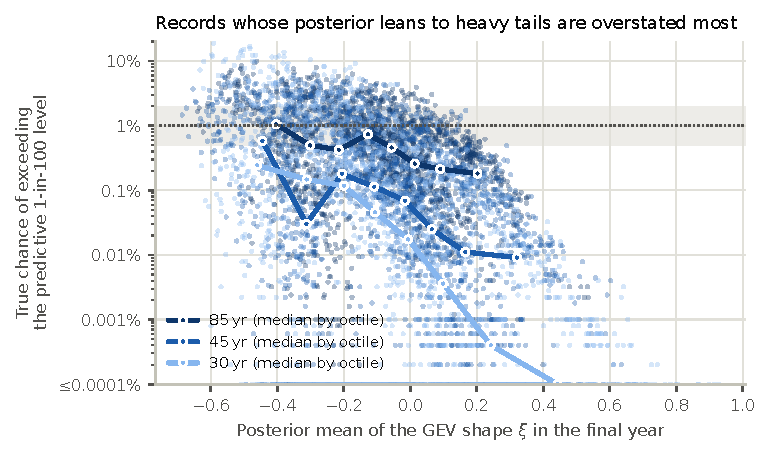
\includegraphics[width=0.75\textwidth]{figures/pred_xi.pdf}
\caption{Records whose posterior leans towards heavy tails are overstated most. One dot per record (standard cases, 30, 45 and 85 years): the true probability that the last year's annual maximum exceeds the posterior-predictive 1-in-100-year level (log scale; ideal 1\%, grey band 0.5--2\%) against the posterior mean of the GEV shape $\xi$ in the last year (larger $\xi$: heavier tail). Lines: medians within eighths of the records sorted by $\xi$. The true $\xi$ of the annual maxima lies between about $-0.25$ and $+0.17$ in all our climates.}\label{fig:pred-xi}
\end{figure}

\paragraph{The prior.}\label{sec:pred-prior}

The predictive level is ``unique'' only for a given prior, and the prior matters a great deal.
Shrinking the prior scales of the random walks from the authors' values (1, 0.5, 0.5) to 0.25
changes nothing about the data, but:
\begin{itemize}
\item at 85 years the share missed falls from 68\% to 57\% (now within 1 point of the posterior
  median and the location trend), and the median true exceedance rises from 0.39\% to 0.64\%;
\item at 45 years the share missed falls from 84\% to 74\% and the median true exceedance rises from
  0.05\% to 0.24\%; record by record the true exceedance of the predictive level rises by a median
  factor of 2.8 (85 years: 1.6);
\item in the cases where the spread and tail follow a rising mean, at 85 years, the predictive level
  with the tight prior becomes the best estimator we tested, missing in 55\% of records against 64\%
  for the Akaike-weighted average and 69\% for the posterior median.
\end{itemize}
We varied only the random-walk scales. The prior on $\xi$ itself, and its upper limit of 2.1, are
likely to matter as much, because the overstatement comes from heavy-tailed draws.

\paragraph{Monte Carlo error.}

Splitting each fit's 4,000 draws into its four chains, the predictive level's chance of being
exceeded changes by a typical factor of 1.06 at 85 years and 1.10--1.11 at 30--45 years (90th
percentile 1.16--1.55). With the authors' 40,000 draws these factors would shrink by about
$\sqrt{10}$. Monte Carlo error accounts for well under 1\% of the variance of the error in the
log exceedance probability (0.03--0.11\%): the dominance of a few draws is a property of the posterior, not of
the number of draws.

\subsection{Ambiguity in the climate, or in the inference?}\label{sec:pred-ambiguity}

One argument for the predictive approach is that possible non-stationarity, combined with possibly
long tails, makes the climate distribution genuinely ambiguous, and that the high and volatile
estimates of catastrophic risk reflect that ambiguity. The synthetic records let us separate the
two parts, because in the no-change cases nothing is changing and the true tail is at most moderately heavy
($\xi\lesssim0.2$):

\begin{table}[H]
\centering\small
\caption{Records with no change at all (the four parents, 100 records each, so 400 per design). Left: median and 10th and 90th percentiles over records of the true probability that the last year's annual maximum exceeds the posterior-predictive 1-in-100-year level (ideal 1\%). Right: share of records (\%) in which the level misses the true risk by more than a factor of 2 either way (true exceedance above 2\% or below 0.5\%), for the predictive level, the Bayesian posterior median and a location-trend fit. Tight prior: random-walk prior scales 0.25. With no change at all, the predictive level is as high and as variable as in the cases with change.}\label{tab:pred-null}
\begin{tabular}{l rrr rrr}
\toprule
 & \multicolumn{3}{c}{Bayes, predictive} & \multicolumn{3}{c}{Missed $>2\times$} \\
\cmidrule(lr){2-4}\cmidrule(lr){5-7}
Design & median & 10\% & 90\% & predictive & post.\ median & loc.\ trend \\
\midrule
30 yr & 0.02\% & 0.00\% & 1.35\% & 89 & 73 & 73 \\
45 yr & 0.08\% & 0.00\% & 1.46\% & 80 & 65 & 66 \\
85 yr & 0.47\% & 0.04\% & 2.31\% & 64 & 53 & 49 \\
85 yr, tight prior & 0.68\% & 0.12\% & 2.30\% & 52 & 48 & 49 \\
\bottomrule
\end{tabular}
\end{table}

With no change at all, the predictive level is as high and as dispersed as in the cases with
change. So most of the ambiguity is produced by the inference: a few decades of annual maxima
cannot rule out a heavy tail, the prior allows one, and averaging probabilities over the posterior
turns that possibility into a high level. That is a legitimate feature of a Bayesian learner's
beliefs, and it is real ambiguity for someone who must act on a short record. But it would be
present in a stationary climate, it shrinks with record length roughly as the tail becomes
identifiable, and its size is governed by prior choices that the data cannot check. It is not, by
itself, evidence that the climate's extremes are changing or are heavy-tailed.

\subsection{Suggestions for practice}\label{sec:pred-suggest}

\begin{enumerate}
\item \textbf{Report the spread of beliefs, not only the average.} Alongside the predictive level,
  report the posterior distribution of the chance of exceeding it, for example the median draw and
  a 90\% range (in our records typically $\sim$0.2\% and 0--5\% at 85 years). That makes clear that
  ``1\%'' is an average over beliefs ranging from negligible to several times the target.
\item \textbf{Show prior sensitivity.} Refit with tighter random-walk scales and a more
  informative prior on $\xi$ (or a lower upper bound), and report how the level and the implied
  premium move. In our records, the random-walk scales alone change the typical true exceedance
  by a factor of 1.6 (85 years) to 2.8 (45 years).
\item \textbf{Benchmark against a stationary climate.} Fit the model to synthetic stationary
  records of the same length and similar distribution. The spread of predictive levels obtained
  there is the ambiguity that comes from the inference alone.
\item \textbf{Compare with simple fits.} If the predictive level is far above both a constant and a
  trend maximum-likelihood fit, the difference comes from the posterior's heavy-tailed draws, and
  should be justified on other grounds (physical or regional knowledge of the tail).
\item \textbf{Bring in more information on the tail.} Pooling the shape parameter across nearby
  stations (regional frequency analysis), or using several values per year, constrains $\xi$
  better than a single annual-maximum record, and the overstatement shrinks as $\xi$ is pinned down.
  In our records, three values per year from 45 years constrained $\xi$ about as well as 85 years
  of annual maxima, but the predictive level still missed in 78\% of records against 68\%; at
  85 years it did slightly less than the tight prior (60\% missed against 57\%). Pooling across
  stations is likely to do more.
\item \textbf{Separate the risk margin from the estimate.} The predictive approach builds a loading
  for ambiguity into the estimate through the prior. If a margin for ambiguity is wanted, it may be
  clearer to estimate the risk with a well-calibrated central estimate and add an explicit,
  stated margin, so that the margin is a decision rather than a by-product of the prior.
\end{enumerate}

%=====================================================================================
\section{Limitations}

\begin{itemize}
\item The synthetic data have no seasonal cycle, a single AR(1) dependence structure, and changes
  that are smooth or a single step. Real daily data have seasonality, longer memory and
  clustering of extremes, which would mostly make things harder.
\item The covariate-model cases are, by construction, cases where that model is right, and the
  covariate is the local mean of the same series. With an external covariate (e.g.\ global mean
  temperature) the gain would depend on how closely the local extremes follow it.
\item 100 records per case gives standard errors of 1--2 percentage points on shares pooled over
  the standard cases and about 5 points for a single case. Estimators are compared on the same records,
  so the differences between them are more precise (about $\pm1$ point pooled), but they depend on
  which cases we chose; differences of a few points should not be over-interpreted.
\item Our MCMC runs are shorter than the authors' (4 $\times$ 1,000 against 4 $\times$ 10,000
  draws). The accuracy of point estimates and interval coverage should be robust to this; the
  convergence failures with three values per year are not a matter of chain length.
\item We scored the final year of each record (a ``nowcast''); a forecast for future years would
  add the uncertainty of extrapolating the random walks. For the Bayesian model we varied only the
  random-walk scales of the prior, not the prior on $\xi$ or its upper limit of 2.1, which matter
  for the predictive level (Section~\ref{sec:pred}).
\item We have not yet run the paper's joint $L^*$ test, the exceedance (threshold) versions of
  the tests, or the Bayes factors that compare ``more events'' with ``a shifted distribution''.
\end{itemize}

%=====================================================================================
\section{Summary}\label{sec:summary}

\emph{What we did.} We reimplemented the time-varying-extremes methods of M\"uller and Watson (2024)
in Python, reproduced their published estimates and test statistics, and tested the methods on
synthetic data for which the truth is known exactly. Daily series were drawn from four parent
distributions (normal; gamma, precipitation-like; Student-$t$, heavy-tailed; beta, bounded) with
day-to-day correlation, and their mean, width or tail was changed over records of 30 to 150 years.

\emph{False alarms.} With one value per year, all the tests we examined keep their nominal 5\%
false-alarm rate, except that the conventional location-trend likelihood-ratio test is over-sized
(7--10\%) for 30-year records. Using the three or ten largest values per year from a persistent
daily series raises false alarms to 20--50\% unless the extremes are declustered.

\emph{Power.} Power rises steeply with record length and is much lower for skewed or heavy-tailed
parents, whose extremes are noisier relative to the daily variability. With one value per year the
Nyblom test is not the most powerful: the simpler Mann--Kendall rank test detects the simulated
changes about as often or more often in almost every case, and a location-trend test is more
powerful against shifts in location but much less powerful against changes in tail shape. The
Nyblom test gains from using the three or ten largest values per year, which Mann--Kendall cannot
use, provided they are declustered.

\emph{How we scored the estimates.} Detecting a change is not the same as measuring it. We scored
more than a dozen estimators on a question that matters for risk assessment: if the estimated 99\%
annual-maximum level for the most recent year is taken at face value, what is the true probability
that it is exceeded? An ideal estimator gives 1\%. We count an estimate as a miss when that
probability is more than 2\% (risk understated at least twofold) or less than 0.5\% (overstated at
least twofold), and report the two directions separately, because their consequences differ and
estimators trade one for the other.

\emph{The noise floor.} The dominant source of error is not the change but the difficulty of
estimating a 1-in-100 level from a few decades of annual maxima: with no change and a correctly
specified model, 44\% of 85-year records miss (27\% understate, 18\% overstate), and about 70\% of
30- and 45-year records.

\emph{Which estimators do best.} Against this floor, a linear trend in location or in location and
width misses 56\% of 85-year records, and an AIC-weighted average of constant, trend and mean-state
models does best (51\%). With 30 or 45 years all these methods are within a few points of each other
and of the no-change floor.

\emph{The Bayesian model.} The authors' Bayesian random-walk model misses 59\% of 85-year records,
erring more often toward understatement. It shrinks estimated changes toward zero, and its 90\%
credible intervals, while they cover the truth, are 1.3 to 3 times wider than the actual errors.
With three values per year, 10--12\% of its fits fail to converge under the authors' prior.

\emph{The posterior-predictive level.} The 99th percentile of the Bayesian posterior predictive
distribution averages probabilities over the draws, so it is pulled up by the few draws with the
heaviest tails. On average over records it is about right or conservative (true exceedance 0.8\%
at 85 years, 0.4--0.6\% at 30--45), and it understates the risk twofold in only 6--13\% of records.
In a single record it usually overstates the risk: it misses twofold in 68\%, 84\% and 92\% of
records at 85, 45 and 30 years, 9 to 19 points more often than the posterior median or a trend fit.
As a pure premium rate for cover with a true 1\% risk it charges a median 1.7--3.2\%. It is as high
and as dispersed with no change at all, and a tighter prior on the random walks brings it close to
the posterior median; most of its ambiguity is therefore produced by the inference (a heavy tail
that a short record cannot rule out and the prior allows), not by the climate.

\emph{Using the wrong driving variable.} Which model is right depends on the physical process, and
our tests show what happens when the model is wrong. We compared models of the same complexity that
differ only in their driving variable: GEV location and scale linear in time, or linear in a
smoothed annual mean of all daily values. When the distribution's width and tail follow an
accelerating mean state, the time-trend models miss the current risk by more than a factor of 2 in
75--83\% of 85-year records against 65\% for the mean-state model. When the width changes while the
mean stays constant, the mean-state model sees nothing and misses 69\% against 55\%. Fitting a
change that is not there costs about as much: with no change, the location + width and covariate
models miss 55--60\% against 44\% for a constant fit.

\emph{Where the choice matters less.} When the mean moves linearly in time the two kinds of model
coincide. When the mean rises at an increasing rate but the width and tail change linearly in time,
the mean-state model, now with the wrong driver, still does slightly better (64\% against 68\%),
because missing the curvature of the mean costs more than misplacing the width. With 30 years every
model misses 66--87\% of records, so the choice of driving variable is secondary to record length.

\emph{When the driver is unknown.} The data rarely reveal the driver: AIC cannot tell a width change
from a mean change. But an AIC-weighted average of the constant, time-trend and mean-state models
comes within 4 points of the best single model for every true process at 85 years.

\emph{Practical conclusion.} These methods can establish \emph{that} extremes are changing, and in
which direction. Statements about the \emph{size} of the current 1-in-100-year level should carry
wide uncertainty, including the spread between physically plausible models of the change, and are
best based on an average over those models rather than on one of them.

%=====================================================================================
\appendix
\section{Cases and supplementary results}

\begin{table}[H]
\centering
\small
\begin{tabular}{lllr}
\toprule
Set & Parent & Change over the record & $\Delta X_{0.99}$ \\
\midrule
Standard & Normal & no change & +0.00 \\
 & Normal & mean +0.5 sd (linear) & +0.50 \\
 & Normal & mean +0.5 sd (step) & +0.50 \\
 & Normal & width $\times$1.22 (linear) & +0.81 \\
 & Gamma & no change & +0.00 \\
 & Gamma & mean +0.5 sd (linear) & +0.50 \\
 & Gamma & mean +0.5 sd (step) & +0.50 \\
 & Gamma & width $\times$1.22 (linear) & +1.58 \\
 & Gamma & tail: log(shape) +1 (linear) & -1.97 \\
 & Student-t & no change & +0.00 \\
 & Student-t & mean +0.5 sd (linear) & +0.50 \\
 & Student-t & mean +0.5 sd (step) & +0.50 \\
 & Student-t & width $\times$1.22 (linear) & +1.64 \\
 & Student-t & tail: log(shape) +1 (linear) & -8.51 \\
 & Beta & no change & +0.00 \\
 & Beta & mean +0.25 sd (linear) & +0.25 \\
 & Beta & mean +0.25 sd (step) & +0.25 \\
 & Beta & width $\times$1.11 (linear) & +0.28 \\
 & Beta & tail: log(shape) +0.2 (linear) & -0.11 \\
 & Beta & position: log $\alpha$ +0.5 (linear) & +0.07 \\
\midrule
Covariate model & Normal & warming +0.5 sd, width \& tail follow (accel.) & +1.02 \\
 & Normal & warming +0.5 sd, width \& tail follow (linear) & +1.00 \\
 & Gamma & wetter: all quantiles $\times$1.22 (accel.) & +1.94 \\
 & Gamma & wetter: all quantiles $\times$1.22 (linear) & +1.86 \\
 & Gamma & wetter $\times$1.22, heavier tail (accel.) & +2.60 \\
 & Student-t & warming +0.5 sd, width \& tail follow (accel.) & +2.32 \\
 & Beta & warming +0.25 sd, width \& tail follow (accel.) & +0.46 \\
\midrule
Time-driven & Normal & warming +0.5 sd, width \& tail linear in time (accel.) & +1.02 \\
 & Student-t & warming +0.5 sd, width \& tail linear in time (accel.) & +2.32 \\
 & Beta & warming +0.25 sd, width \& tail linear in time (accel.) & +0.46 \\
\bottomrule
\end{tabular}

\caption{Cases of the quantification study. Standard: one feature of the daily distribution changes linearly or in a step. Covariate model: the width and tail follow an accelerating mean state (for the gamma, every quantile scales with the mean). Time-driven: the same first- and last-year distributions as the covariate-model cases, reached linearly in time. Changes: mean in baseline daily sd; width as a factor; tail as the change in log(shape), the log of the gamma shape $a$, the $t$ degrees of freedom $\nu$ or the beta $\beta$ (increasing it lightens the tail of the gamma and $t$); position as the change in $\log\alpha$ of the beta. $\Delta X_{0.99}$: resulting true change in the 1-in-100-year level over an 85-year record (baseline daily sd).}
\label{tab:cases}
\end{table}

\begin{table}[H]
\centering
\small
\begin{tabular}{lrrrrrrr}
\toprule
True process & Const. & Loc. & Loc.+wid. & Bayes & Cov. & AIC & AIC avg. \\
\midrule
\multicolumn{8}{l}{\emph{Understated $>2\times$, 85 years}} \\
No change & \textbf{27} & \textbf{32} & \textbf{36} & \textbf{36} & \textbf{38} & -- & -- \\
Mean shift, linear in time & 61 & \textbf{32} & \textbf{36} & \textbf{44} & \textbf{38} & -- & -- \\
Mean shift, step & 52 & 16 & 19 & \textbf{37} & \textbf{25} & -- & -- \\
Width change, mean constant & 73 & 47 & \textbf{37} & \textbf{50} & 54 & -- & -- \\
Tail change, mean constant & 0 & 25 & 34 & \textbf{21} & 20 & -- & -- \\
Follows mean state, mean linear in time & 80 & 44 & \textbf{36} & \textbf{50} & \textbf{35} & -- & -- \\
Follows mean state, mean accelerating & 89 & 81 & 69 & \textbf{60} & \textbf{49} & -- & -- \\
Follows time, mean accelerating & -- & -- & -- & -- & -- & -- & -- \\
\multicolumn{8}{l}{\emph{Overstated $>2\times$, 85 years}} \\
No change & \textbf{18} & \textbf{17} & \textbf{19} & \textbf{17} & \textbf{23} & -- & -- \\
Mean shift, linear in time & 6 & \textbf{17} & \textbf{19} & \textbf{14} & \textbf{18} & -- & -- \\
Mean shift, step & 6 & 38 & 36 & \textbf{19} & \textbf{19} & -- & -- \\
Width change, mean constant & 2 & 7 & \textbf{18} & \textbf{12} & 15 & -- & -- \\
Tail change, mean constant & 82 & 50 & 25 & \textbf{39} & 47 & -- & -- \\
Follows mean state, mean linear in time & 2 & 8 & \textbf{19} & \textbf{13} & \textbf{17} & -- & -- \\
Follows mean state, mean accelerating & 1 & 2 & 5 & \textbf{12} & \textbf{16} & -- & -- \\
Follows time, mean accelerating & -- & -- & -- & -- & -- & -- & -- \\
\bottomrule
\end{tabular}

\caption{The misses of Table~\ref{tab:wrong} at 85 years split by direction: share of records (\%) with the risk understated at least twofold (top: true probability of exceeding the estimated level above 2\%, so the level is too low) and overstated at least twofold (bottom: below 0.5\%, too high), by true process (rows) and fitted model (columns as in Table~\ref{tab:wrong}). Bold: the model's form contains the true process.}
\label{tab:wrongdetail}
\end{table}

\begin{figure}[H]
\centering
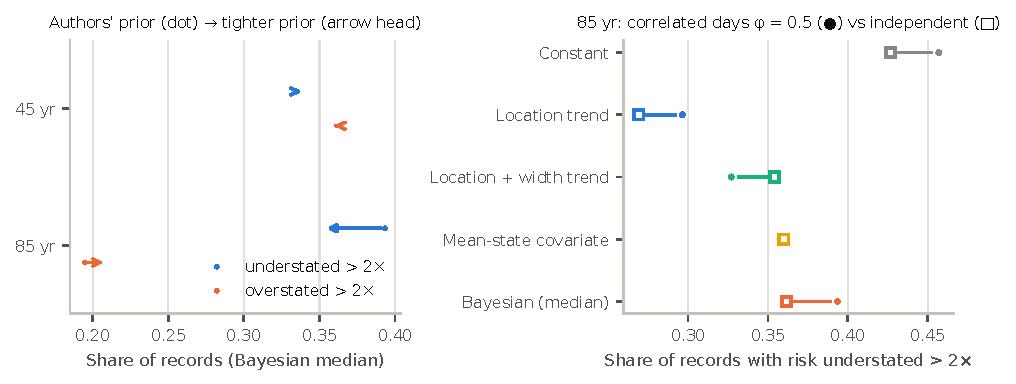
\includegraphics[width=\textwidth]{figures/figA1_prior_phi.pdf}
\caption{Left: effect of a tighter prior on the Bayesian model's random walks (scales 0.25 instead of the authors' 1, 0.5, 0.5) at 45 and 85 years: share of records whose posterior-median 1-in-100-year level understates (blue) or overstates (red) the risk at least twofold (true probability of exceeding it above 2\% or below 0.5\%); dot: authors' prior; arrow head: tighter prior. Right: share of 85-year records missed by more than a factor of 2 either way, by estimator, with correlated ($\phi=0.5$, dot) and independent (square) daily values. The tighter prior reduces understatement at 85 years; independent days make every estimator slightly worse.}
\label{fig:prior}
\end{figure}

\section{The posterior-predictive level at 30 years by kind of change}

\begin{table}[H]
\centering\small\setlength{\tabcolsep}{3.5pt}
\caption{The posterior-predictive level at 30 years, by kind of change and by parent distribution, with the columns of Table~\ref{tab:pred-groups}: median true exceedance probability (ideal 1\%), shares (\%) understated (true exceedance above 2\%, level too low) and overstated (below 0.5\%, level too high) at least twofold, and missed; right, missed by other estimators on the same records. At 30 years the predictive level overstates the risk in 78--92\% of records in every kind of case.}
\begin{tabular}{l r rrr r rrr}
\toprule
 & & \multicolumn{4}{c}{Bayes, predictive} & \multicolumn{3}{c}{Missed, others} \\
\cmidrule(lr){3-6}\cmidrule(lr){7-9}
Kind of change & records & median & under & over & \textbf{missed} & \shortstack{post.\\median} & \shortstack{loc.\\trend} & \shortstack{AIC\\avg.} \\
\midrule
No change & 400 & 0.02\% & 7 & 82 & \textbf{89} & 73 & 73 & 74 \\
Mean & 800 & 0.01\% & 9 & 84 & \textbf{92} & 75 & 69 & 72 \\
Width & 400 & 0.02\% & 10 & 81 & \textbf{91} & 77 & 76 & 79 \\
Tail & 300 & 0.01\% & 3 & 92 & \textbf{95} & 73 & 79 & 74 \\
Position (beta) & 100 & 0.00\% & 7 & 88 & \textbf{95} & 80 & 76 & 77 \\
Follows mean state & 700 & 0.01\% & 9 & 78 & \textbf{87} & 80 & 83 & 82 \\
Time-driven & 300 & 0.01\% & 9 & 81 & \textbf{90} & 78 & 83 & 81 \\
\midrule
Normal (standard cases) & 400 & 0.01\% & 8 & 82 & \textbf{90} & 75 & 72 & 76 \\
Gamma (standard cases) & 500 & 0.02\% & 7 & 84 & \textbf{91} & 72 & 70 & 73 \\
Student-t (standard cases) & 500 & 0.04\% & 7 & 84 & \textbf{91} & 73 & 70 & 69 \\
Beta (standard cases) & 600 & 0.00\% & 8 & 87 & \textbf{95} & 79 & 79 & 80 \\
\bottomrule
\end{tabular}

\end{table}

\section*{References}
\begin{list}{}{\leftmargin=1.5em \itemindent=-1.5em \itemsep=0.2em}
\item Carpenter, B., et al. (2017). Stan: a probabilistic programming language. \emph{Journal of
  Statistical Software} 76(1).
\item Coles, S. (2001). \emph{An Introduction to Statistical Modeling of Extreme Values}. Springer.
\item M\"uller, U. K. and M. W. Watson (2024). Time varying extremes. \emph{Review of Economics and
  Statistics}, doi:10.1162/rest\_a\_01528.
\item Nyblom, J. (1989). Testing for the constancy of parameters over time. \emph{Journal of the
  American Statistical Association} 84, 223--230.
\item Philip, S., et al. (2020). A protocol for probabilistic extreme event attribution analyses.
  \emph{Advances in Statistical Climatology, Meteorology and Oceanography} 6, 177--203.
\end{list}

\end{document}
